\documentclass[x11names]{report}
\usepackage[a4paper, total={6in, 9in}]{geometry}
\usepackage[skins]{tcolorbox}
\usepackage{tikz}
\usetikzlibrary{arrows}
\usetikzlibrary{calc}
\usepackage{pgfplots}
\pgfplotsset{compat=1.9}
\usepgflibrary{shapes.geometric}
\usepackage{xcolor}
\usepackage{amsmath}
%\usepackage{fouriernc}
\usepackage{mathrsfs}
\usepackage{amssymb}
\usepackage{hyperref}
\usepackage{graphicx,import}
\usepackage{float}
\usepackage{wrapfig}
\usepackage{multicol}
\usepackage{cancel}
\setlength{\columnsep}{1cm}

%% custom
\renewcommand*\contentsname{Indice}
\setcounter{tocdepth}{2}
\setcounter{secnumdepth}{2}
\pgfplotsset{compat=1.15}

\usepackage[pagestyles]{titlesec}
\titleformat{\chapter}[display]{\normalfont\bfseries}{}{0pt}{\Huge}
\newpagestyle{mystyle}
{\sethead[\thepage][][\chaptertitle]{}{}{\thepage}}
\pagestyle{mystyle}


% boxes
\definecolor{myblue}{RGB}{224, 245, 255} 
\definecolor{myred}{RGB}{198, 247, 211} 
\definecolor{myorange}{RGB}{255, 102, 0} 
\definecolor{mypurple}{RGB}{255, 102, 0} 
\definecolor{attenzione}{RGB}{255, 108, 94}

\newtcolorbox{es}[2][]{%
	enhanced,sharp corners,boxrule=0.4pt,colback=white, colframe=black, coltitle=black,fonttitle=\itshape, 
	attach boxed title to top left={yshift=-0.5\baselineskip-0.4pt,xshift=2mm},
	boxed title style={tile, size=minimal, left=0.5mm, right=0.5mm,
		colback=white, before upper=\strut, boxrule=0.5pt, colframe=black},
	title=#2,top=1em,#1 
}
\newtcolorbox{dym}[2][]{%
	enhanced,colback=white,colframe=black,coltitle=black,
	sharp corners,boxrule=0pt, %0.4pt
	fonttitle=\itshape,,
	attach boxed title to top left={yshift=-0.5\baselineskip-0.4pt,xshift=2mm},
	boxed title style={tile,size=minimal,left=2.5mm,right=0.5mm,
		colback=white,before upper=\strut},
	title=#2,top=1em,#1
}
\newtcolorbox{blues}[2][]{%
	enhanced,colback=myblue,colframe=black,coltitle=black,
	sharp corners,boxrule=0.4pt,
	fonttitle=\bfseries\itshape,
	attach boxed title to top left={yshift=-0.5\baselineskip-0.4pt,xshift=2mm},
	boxed title style={tile,size=minimal,left=0.5mm,right=0.5mm,
		colback=myblue,before upper=\strut},
	title=#2,top=1em,#1
}
\newtcolorbox{redes}[2][]{%
	enhanced,colback=myred,colframe=black,coltitle=black,
	sharp corners,boxrule=0.4pt,
	fonttitle=\bfseries\itshape,
	attach boxed title to top left={yshift=-0.5\baselineskip-0.4pt,xshift=2mm},
	boxed title style={tile,size=minimal,left=0.5mm,right=0.5mm,
		colback=myred,before upper=\strut},
	title=#2,top=1em,#1
}
\newtcolorbox{coroll}[2][]{%
	enhanced, colback=white, colframe=black, coltitle=black,
	sharp corners, boxrule=0pt,
	fonttitle=\bfseries\itshape,
	attach boxed title to top left={yshift=-0.5\baselineskip-0.4pt,xshift=2mm},
	boxed title style={tile,size=minimal,
		left=1mm, right=1mm, % Horizontal padding
		top=1mm, bottom=1mm, % Vertical padding
		colback=myred,
		before upper=\strut},
	title=#2,top=1em,#1
}
\newtcolorbox{attenzione}[2][]{%
	enhanced,colback=white,colframe=attenzione,coltitle=attenzione,
	sharp corners,boxrule=0.4pt,
	fonttitle=\itshape,
	attach boxed title to top left={yshift=-0.5\baselineskip-0.4pt,xshift=2mm},
	boxed title style={tile,size=minimal,left=0.5mm,right=0.5mm,
		colback=white,before upper=\strut},
	title=#2,#1
}

\newcommand*{\QEDA}{\null\nobreak\hfill\ensuremath{\blacksquare}}%
\newcommand*{\QEDB}{\null\nobreak\hfill\ensuremath{\square}}%

\newcommand{\esempio}[2]{
	\begin{es}{#1}
		#2
	\end{es}
}
\newcommand{\definizione}[2]{
	\begin{center}
		\fboxsep11pt
		\colorbox{myblue}{\begin{minipage}{5.75in}
				\begin{blues}{Definizione: #1}
					#2
				\end{blues}
		\end{minipage}}
	\end{center}
}
\newcommand{\teorema}[2]{
	\begin{center}
		\fboxsep11pt
		\colorbox{myred}{\begin{minipage}{5.75in}
				\begin{redes}{#1}
					#2
				\end{redes}
		\end{minipage}}
	\end{center}
}
\newcommand{\dimostrazione}[2]{
	\begin{dym}{dimostrazione#1}
		#2
		\QEDB
	\end{dym}
}
\newcommand{\corollario}[2]{
	\begin{center}
		\begin{coroll}{corollario#1}
			#2
		\end{coroll}
	\end{center}
}
\newcommand{\nota}[2]{
	\begin{attenzione}{Nota:}
		#2
	\end{attenzione}
}

\newcommand{\mathbox}[1]{
\begin{tcolorbox}[rounded corners, colback=blue!5, colframe=blue!80!black, title=Formule Matematiche]
	#1
\end{tcolorbox}
}



% svg + latex
\usepackage{import}
\usepackage{xifthen}
\usepackage{pdfpages}
\usepackage{transparent}

\newcommand{\incfig}[1]{%
	\import{./img/}{#1.pdf_tex}
}
\newcommand{\viola}[1]{%
	\colorbox{myblue}{$\displaystyle #1$}
}
\newcommand{\rosso}[1]{%
	\colorbox{myred}{$\displaystyle #1$}}

\pgfplotsset{my axis/.append style={height=9cm,width=9cm,grid=major,samples=100,yticklabel=\empty,xticklabel=\empty}}
\pgfplotsset{my plot/.append style={thick,samples=500}}

\begin{document}
	
\begin{titlepage}
	\begin{center}
		\vspace*{1cm}
		
		\textbf{\LARGE Relazione di laboratorio - Pendolo semplice}
		
		\vspace{0.3cm}
		\large \textit{Misura del periodo di un pendolo semplice} \\
		
		\vspace{0.5cm}
		\Large Federico Cesari \\
		
		\small 1096759 
		\vspace{0.2cm}
		
		\small Gruppo 5
		
		
		\vspace{3cm}
		\begin{center}
			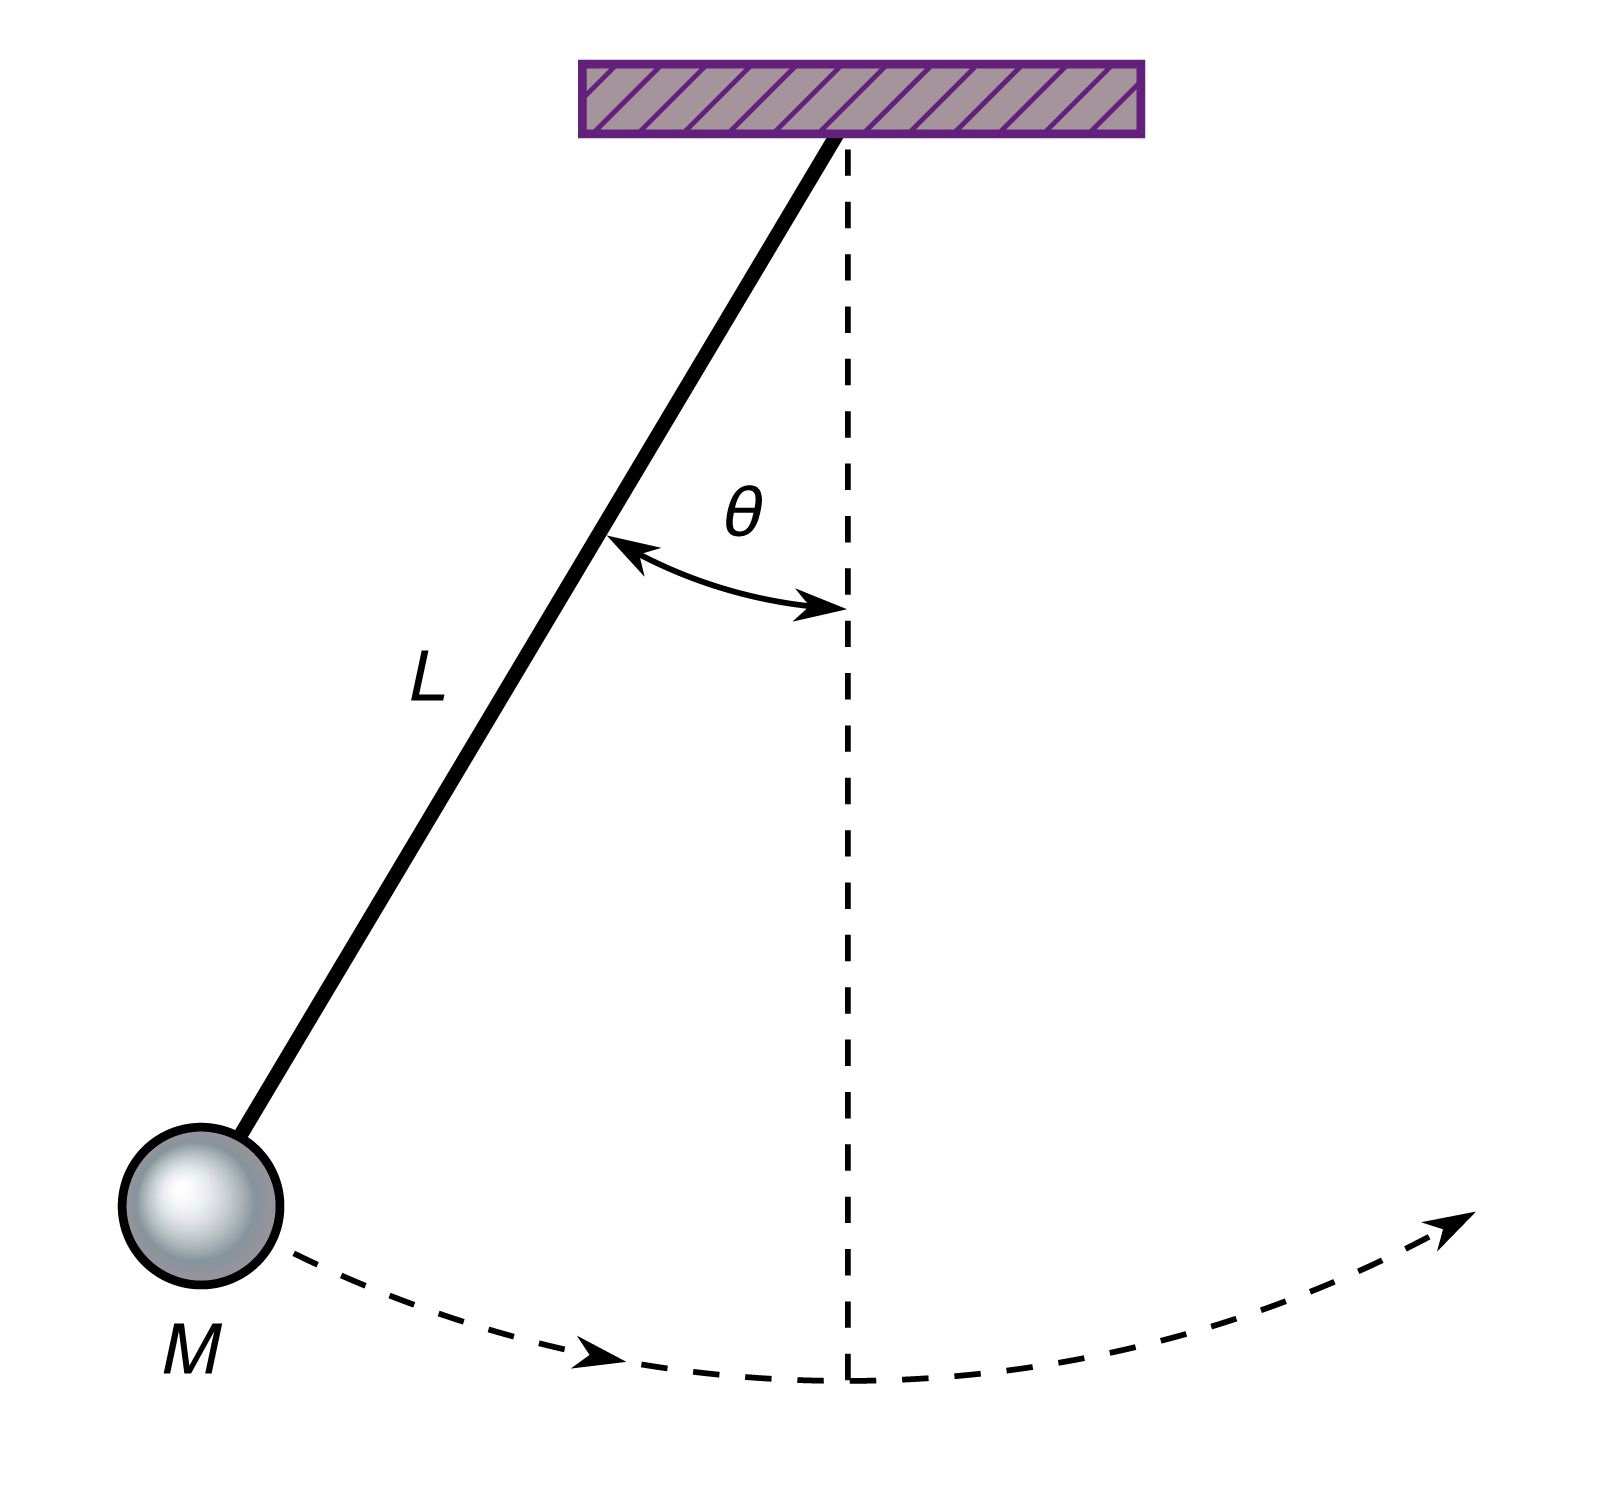
\includegraphics[scale=0.1]{IMG_0200.jpeg}	
		\end{center}
		
		
		
		\vfill
		
		
		
		corso A\\
		Università degli studi di Torino, Torino\\
		4 aprile 2024\\
		
		
	\end{center}
\end{titlepage}
\tableofcontents
\newpage
	
\chapter{Elettrostatica}
\section{Campo elettrostatico}
\definizione{Campo elettrostatico}{
Il campo elettrostatico prodotto in un punto \(P\) da un sistema di cariche ferme è definito come forza elettrostatica risultante \(F\) che agisce su una carica di prova \(q_0\) posta in \(P\) divisa per la carica stessa.
}
In realtà la carica di prova può perturbare la distribuzione di cariche originale, per questo la definizione diventerebbe più precisa se si facesse tendere a zero il valore di \(q_0\). In pratica è sufficiente che \(q_0\) sia molto piccola rispetto alle altre cariche.
\subsection{Dipolo elettrico}
Definiamo \textbf{momento del dipolo}
\begin{equation}
	\viola{\vec{p} = q\vec{a}}
\end{equation}


Consideriamo un punto \(P\) nel quale misuriamo il potenziale, pari alla somma dei contributi delle due cariche:
\[
V(P) = \frac{q}{4\pi \varepsilon_0} \left(\frac{1}{r_1} - \frac{1}{r_2}\right) = \frac{q}{4\pi \varepsilon_0} \left(\frac{r_2 - r_1}{r_1r_2}\right)
\]
Ipotizziamo che \(P\) sia molto distante dal dipolo (rispetto alla distanza \(a\)) così che \(r_1\) e \(r_2\) siano sempre più assimilabili a due segmenti paralleli. Andiamo poi a tracciare un segmento perpendicolare a \(r_1\) fino a \(r_2\) evidenziando la distanza \(r_2 - r_1 \approx a\cos\vartheta\). 

\subsubsection{Potenziale del dipolo}
Con le seguenti approssimazioni andiamo a riscrivere il potenziale:
\[
r_2 - r_1 \approx a\cos\vartheta \qquad \qquad r_1r_2 \approx r^2
\]
\[
V(P) = \frac{q}{4\pi \varepsilon_0} \left(\frac{a\cos\vartheta}{r^2}\right) = \frac{p}{4\pi \varepsilon_0 r^2}
\]
\begin{equation}
	\viola{V(P) =\frac{p}{4\pi \varepsilon_0 r^2}}
\end{equation}
Vediamo come a grandi distanze il potenziale del punto \(P\) dia \textit{informazioni solo sul momento di dipolo} e non sulle due cariche o sulla loro distanza reciproca. A parità di momento si potranno avere due cariche ravvicinate e molto cariche o più distanti e meno cariche.


\subsubsection{Campo elettrico del dipolo}
Riscrivendo \(r\) e \(\cos\vartheta\) esprimiamo il potenziale come
\[
V(P) = \frac{q}{4\pi \varepsilon_0} \left(\frac{a\textcolor{orange}{\cos\vartheta}}{\textcolor{red}{r^2}}\right) 
\]
\[
V(P)= \frac{p}{4\pi\varepsilon_0}\frac{1}{\textcolor{red}{x^2 + y^2 + z^2}}\textcolor{orange}{\frac{z}{\sqrt{x^2 + y^2 + z^2}}} = \frac{p}{4\pi\varepsilon_0}\frac{z}{(x^2+y^2+z^2)^{\frac{3}{2}}}
\]\\

\noindent
Dalla relazione \(\vec{E} = -\vec{\nabla}V\) otteniamo l'espressione del campo elettrico
\[
\vec{E} = \left( \frac{p}{4\pi\varepsilon_0}\frac{3xz}{r^5},\;\ \frac{p}{4\pi\varepsilon_0}\frac{3yz}{r^5},\;\ \frac{p}{4\pi\varepsilon_0}\left(\frac{3z^2}{r^5}-\frac{1}{r^3}\right)\right) 
\]
\begin{equation}
	\viola{E(P) = \frac{p}{4\pi\varepsilon_0r^3}\sqrt{3\cos^2\vartheta + 1}}
\end{equation}
Concludiamo osservando che il campo elettrico del dipolo varia con \(r^3\) (il monopolo con \(r^2\)) e dipende anche dall'angolo \(\vartheta\).


\section{Lavoro elettrico}
Quando su una carica \(q_0\) agisce una forza \(\vec{F}\) \textit{di qualsiasi natura}, possiamo definire sempre un campo elettrico \(\vec{E}\) che chiamiamo \textbf{campo elettromotore}
\[
\vec{E} = \frac{\vec{E}}{q_0} \;\ \to \;\ \vec{F} = q_0 \vec{E}
\]
di cui non conosciamo necessariamente la natura; nel caso di un insieme di cariche ferme questo coinciderà con il campo elettrostatico, ma in questo caso studiamo il caso più generale.

Suddividendo il percorso da \(A\) a \(B\) in segmenti infinitesimi \(d\vec{s}\) calcoliamo il lavoro come integrale di linea del campo \(E\) lungo \(C_1\) 

\[
dW_1 = \vec{F}\cdot d\vec{s} = q_0\vec{E} \cdot d\vec{s}
\]
\[
 W_1 =  q_0 \int_{C_1} \vec{E} \cdot d\vec{s}
\]

\subsection{Tensione elettrica e forza elettromotrice}
\definizione{Tensione elettrica}{
Il rapporto tra il lavoro compiuto dalla forza \(\vec{F}\) nello spostamento da \(A\) a \(B\) lungo il percorso \(C_1\) e la carica 


\begin{equation}
	T(A\to B,C_1) \;\ = \;\ \frac{W_1}{q_0} \;\ =\;\ \int_{C_1}\vec{E}\cdot d\vec{s}
\end{equation}

viene definito \textbf{tensione elettrica}.
}
Se si considera un secondo percorso \(C_2\) si trova in generale un lavoro diverso e quindi un diverso valore della tensione elettrica pur essendo i punti \(A\) e \(B\) gli stessi.


Se studiamo il lavoro lungo un percorso chiuso invece troviamo
\[
W = \oint \vec{F} \cdot d\vec{s} = q_0\oint\vec{E}\cdot d\vec{s}
\]
\definizione{Forza elettromotrice}{
Il rapporto tra lavoro compiuto sulla carica e la carica stessa per il percorso chiuso, ovvero l'integrale di linea circuitazione di campo elettrico
\begin{equation}
\mathcal{E} = \oint\vec{E}\cdot d\vec{s}
\end{equation}
viene definito \textbf{forza elettromotrice} relativa al percorso chiuso \(C\).
}
Sviluppando l'integrale
\begin{align*}
	\oint\vec{F}\cdot d\vec{s} =& \int_{C_1}\vec{F}\cdot d\vec{s} + \int_{-C_2}\vec{F}\cdot d\vec{s} \\
							   =& \int_{C_1}\vec{F}\cdot d\vec{s} - \int_{C_2}\vec{F}\cdot d\vec{s} \\
							   =& W_1 - W_2
\end{align*}
vediamo che in generale per un percorso chiuso il lavoro è diverso da zero. Tuttavia andremo a studiare il comportamento del \textit{campo elettrostatico} che è conservativo e di conseguenza ha circuitazione nulla. 


\subsection{Potenziale elettrostatico ed energia potenziale}
Se il campo è conservativo, non dipendendo dal percorso  seguito l'espressione della tensione elettrica può essere riscritta semplicemente come l'integrale tra \(A\) e \(B\) 
\[
\int_{A}^B\vec{E}\cdot d\vec{s} = f(B) - f(A)
\]
dove \(f\) è una particolare funzione definita a meno di una costante arbitraria e che rinominiamo \(V\) \textbf{potenziale elettrostatico}. 
\definizione{Differenza di potenziale elettrostatico}{
Possiamo definire una \textbf{differenza di potenziale} pari a 
\begin{equation}
\Delta V = - \int_{A}^B\vec{E}\cdot d\vec{s} 
\end{equation}
}
Ricordando che ad ogni forza conservativa è associata una determinata energia potenziale e che il lavoro della forza conservativa è pari all'opposto della variazione della corrispondente energia potenziale
\[
W = -\Delta U_e
\]
\textit{Sono riportate in appendice alcune precisazioni sulle definizioni di potenziale elettrostatico e di energia potenziale (\ref{precisazioni potenziale})}. \\


\noindent
Dalle definizioni precedenti possiamo scrivere le seguenti relazioni
\[
W = q_0 \mathcal{E}  \qquad\qquad \Delta U_e = q_0 \Delta V
\]
\[
W = -q_0 \Delta V \qquad\qquad  \Delta U_e = - q_0 \mathcal{E}
\]

\dimostrazione{: il "campo elettrostatico è conservativo"}{
	Dimostriamo che il campo elettrostatico di una qualsiasi distribuzione di carica è conservativo; cominciamo dal caso più semplice del campo generato da una carica puntiforme:
	\[
	dW = \boldsymbol{q_0}\vec{E} \cdot d\vec{s} = \frac{\boldsymbol{q_0}q}{4\pi\varepsilon_0} \frac{\hat{u}_r \cdot d\vec{s}}{r^2} =  \frac{\boldsymbol{q_0}q}{4\pi\varepsilon_0} \frac{dr}{r^2}
	\]
	Si ottiene che il lavoro da \(A\) a \(B\), caratterizzati dalle distanze \(r_A\) e \(r_B\) dall'origine, vale
	\begin{align*}\label{sviluppo lavoro}
		W =&  \frac{\boldsymbol{q_0}q}{4\pi\varepsilon_0} \int_A^B  \frac{dr}{r^2} \\
		=& -\left(\frac{q_0 q}{4\pi \varepsilon_0 r_B} - \frac{q_0 q}{4\pi \varepsilon_0 r_A}\right)
	\end{align*}
	indipendente dal percorso seguito.
}

\section{Flusso di campo elettrico}
Definiamo flusso di un campo vettoriale \(\vec{E}\) l'integrale
\[
\Phi (\vec{E}) = \int_{\Sigma} \vec{E}\cdot \hat{u}_n \: d\Sigma
\]
dove \(\hat{u}_n\) è il versore normale alla porzione infinitesima di superficie \(d\Sigma\). Vediamo che il prodotto scalare fa sì che contribuisca solo la componente di campo vettoriale ortogonale alla superficie. 

\begin{figure}[h]
	\centering
	\incfig{gauss_subs_1}
\end{figure}

Mostriamo come il flusso \textit{dipenda solo dall'angolo solido sotto il quale la superficie vede la carica}. Prima di tutto qualche osservazione geometrica:

\[
d\vartheta = \frac{ds}{r} \qquad \qquad ds' \cos\alpha = ds \;\ \to \;\ d\vartheta = \frac{ds'\cos\alpha}{r}
\]
\[
d\Omega= \frac{d\Sigma_0}{r^2} \qquad \qquad d\Sigma \cos\alpha = d\Sigma_0 \;\ \to \;\ d\Omega = \frac{d\Sigma\cos\alpha}{r^2}
\]

\begin{figure}[h]
	\centering
	\incfig{gauss_1}
\end{figure}


Andiamo ora a calcolare il flusso attravgausserso \(d\Sigma\):
\begin{align*}
	d\Phi =& \vec{E} \cdot \hat{u}_n d\Sigma \\ 
		  =& \frac{q}{4\pi\varepsilon_0 r^2} \hat{u}_r \cdot \hat{u}_n \: d\Sigma \\
		  =& \frac{q}{4\pi\varepsilon_0 r^2} |\hat{u}_r||\hat{u}_n|\textcolor{red}{\cos\alpha\: d\Sigma} \\ 
		  =& \frac{q}{4\pi\varepsilon_0 r^2} |\hat{u}_r||\hat{u}_n|\textcolor{red}{\: d\Sigma_0} \\
		  =& \frac{q}{4\pi\varepsilon_0  \textcolor{orange}{r^2}} \textcolor{orange}{\: d\Sigma_0} \\
		  =& \frac{q}{4\pi\varepsilon_0}\: \textcolor{orange}{d\Omega} \quad \to \quad \Phi = \frac{q}{4\pi\varepsilon_0}\Omega
\end{align*}
Quindi se consideriamo una superficie chiusa si ha un angolo solido 
\[
d\Omega = \frac{4\pi r^2}{r^2} = 4\pi
\]
e di conseguenza
\begin{equation}
	\viola{\Phi = \frac{q}{\varepsilon_0}}
\end{equation}
Se la carica esterna il flusso è nullo (le cariche esterne contribuiscono solo al campo elettrico). Inoltre se consideriamo più cariche, o addirittura una distribuzione omogenea di cariche si hanno i seguenti valori di flusso:
\[
\text{distribuzione finita di cariche: }\qquad \Phi = \oint \vec{E} \cdot \hat{u}_n \: d\Sigma \;\ = \;\ \sum_i \frac{q_{i(int)}}{\varepsilon_0}
\]
\[
\text{distribuzione continua di cariche: }\qquad \Phi = \frac{1}{\varepsilon_0}\int \rho(x,y,z) \:d\tau 
\]




\subsection{Rotore di un campo vettoriale}
Viene definito rotore del campo elettrico \(\vec{E}\) il prodotto vettoriale
\[
\vec{\nabla} \wedge \vec{E} = \left|\begin{array}{ccc}
	\hat{u}_x & \hat{u}_y & \hat{u}_z \\
	\frac{\partial}{\partial x} & \frac{\partial}{\partial y} & \frac{\partial}{\partial z} \\
	E_x & E_y & E_z 
\end{array}\right| = \left(\frac{\partial E_z}{\partial y}-\frac{\partial E_y}{\partial z}\right)\hat{u}_x + \left(\frac{\partial E_x}{\partial z}-\frac{\partial E_z}{\partial x}\right)\hat{u}_y + \left(\frac{\partial E_y}{\partial x}-\frac{\partial E_x}{\partial y}\right)\hat{u}_z
\]
Questo rappresenta la capacità del campo elettrico di \textit{formare vortici}, ovvero di generare linee di forza che si richiudono su loro stesse.


Poiché anche il rotore del campo elettrico è un campo vettoriale, è possibile definirne un suo flusso:

\[
\Phi(\vec{\nabla} \wedge \vec{E}) =  \int_{\Sigma}\left(\vec{\nabla} \wedge \vec{E}\right)\cdot \hat{u}_n \: d\Sigma
\]

\teorema{}{\label{stokes}
\subsubsection{Teorema di Stokes}
La circuitazione è uguale al flusso del rotore:
\[
\oint_{\partial\Sigma} \vec{E}\cdot d\vec{s} = \int_{\Sigma}\left(\vec{\nabla} \wedge \vec{E}\right)\cdot \hat{u}_n \: d\Sigma
\]
Qui è espresso nel caso del campo elettrico dove si ha che la circuitazione è nulla qualunque sia la curva \(\gamma = \partial \Sigma\) (a patto che sia chiusa). Allora il flusso del rotore è nullo qualunque sia la superficie ed è possibile solo se il rotore di \(\vec{E}\) è nullo:

\[
\vec{\nabla} \wedge \vec{E} = 0
\]

Dire che il rotore è nullo equivale a dire che il capo elettrico è \textbf{irrotazionale}, ovvero che le sue linee di forza non possono chiudersi su loro stesse; il campo elettrico "non forma vortici".

\textcolor{gray}{\textit{Vedremo che in presenza di un campo magnetico variabile il rotore del campo elettrico non è più nullo.}}
}

L'annullarsi del rotore non è un fatto sorprendente. Sappiamo infatti che il rotore di un gradiente è sempre nullo e che il campo elettrostatico conservativo può essere scritto come gradiente della funzione scalare del potenziale elettrostatico \(V\):
\[
\vec{\nabla} \wedge \vec{E} = \vec{\nabla} \wedge \left(-\vec{\nabla} V\right)
\]

\subsection{Divergenza di un campo vettoriale}
L'operatore divergenza si applica ad un campo vettoriale e dà origine ad un campo scalare. Il suo significato intrinseco è espresso da 
\begin{equation}
	\viola{d\Phi(\vec{E}) = \vec{\nabla}\cdot\vec{E}\,\ d\tau}
\end{equation}


Prendendo in considerazioni tanti volumetti \(d\tau\) calcoliamo il flusso infinitesimo del campo \(\vec{E}\) attraverso la superficie infinitesima \(d\Sigma\) del volumetto. Estendendo il risultato a tutto il volume \(\tau\) si osserva che i contributi interni al volume si elidono a vicenda e le uniche superfici che contribuiscono al calolo del flusso sono quelle esterne:
\[
\int_\tau d\Phi(\vec{E}) = \int_\tau  \vec{\nabla}\cdot\vec{E}\,\ d\tau = \oint_\Sigma \vec{E}\cdot\hat{u}_n \,\ d\Sigma
\]

\newpage
\section{Conduttori}
\definizione{Materiale conduttore}{
	Un materiale è detto conduttore se l'elettrizzazione conseguente allo strofinio si diffonde rapidamente andando ad interessare anche zone lontane da quelle in cui è stata prodotta. 
}
I materiali conduttori sono caratterizzati dal fatto che nel loro interno sono verificate particolari condizioni per cui è possibile il moto di alcune cariche (positive e negative in gas ionizzati e soluzioni elettrolitiche e negative nei conduttori solidi) che li costituiscono.

Il moto degli elettroni liberi in un conduttore in equilibrio elettrostatico è completamente disordinato ottenendo perciò una velocità media nulla delle cariche. Si andrà quindi ad assumere che le cariche siano fisse all'interno di un conduttore e che di conseguenza il campo elettrico si annulli:
\[
\vec{E} = 0 \qquad\qquad \text{all'interno}
\]
fatto che comporta le seguenti conseguenze:
\begin{enumerate}
	\item \(\Phi(\vec{E}) = 0\) attraverso qualsiasi superficie gaussiana interna al conduttore. L'annullarsi del flusso implica l'annullarsi della carica. Si ha quindi che l'eccesso di carica su un conduttore può esistere solo in superficie con densità superficiale \(\sigma\);
	\item Avendo definito \(\vec{E} = - \vec{\nabla}V\) si ha che il potenziale è costante in tutto il conduttore:
	\[
	V(P_1) - V(P_2) = \int_{P_1}^{P_2}\vec{E} \cdot d\vec{s} = 0 \quad \implies \quad V(P_1) = V(P_2) = V_0
	\]
	dove \(V_0\) corrisponde al lavoro di estrazione.
	Questo fa sì che la superficie del conduttore sia equipotenziale e, quindi, che il campo elettrico sia localmente ortogonale alla superficie (il gradiente è ortogonale alle curve di livello) e valga
	
	\begin{figure}[H]
		\centering
		\incfig{cilindro_piano}
	\end{figure}
	\[
	\Phi(\vec{E}) = 2 E\Sigma = 2 E\pi R^2 = \frac{q}{\varepsilon_0} = \frac{\sigma 2\pi R^2}{\varepsilon_0} \quad \implies \quad \vec{E} = \frac{\sigma}{\varepsilon_0}\hat{u}_n
	\]
\end{enumerate}

\paragraph*{Campo elettrico indotto}
Avvicinando un conduttore carico o scarico ad un altro corpo carico, ovvero introducendolo in un campo elettro esterno \(\vec{E}_\text{est}\) il campo elettrico interno non sarebbe più nullo; senonché questo fatto provoca un movimento di elettroni che si spostano per l'azione del campo elettrico esterno e si accumulano in una zona della superficie, lasciando sul resto della superficie un eccesso di carica positiva: tra queste zone si crea un campo elettrostatico indotto \(\vec{E}_i\) che contrasta il movimento degli elettroni fino a raggiungere l'equilibrio quando
\[
\vec{E}_i + \vec{E} = 0
	\]
\begin{figure}[H]
	\centering
	\incfig{lastre_piastra}
\end{figure}

\subsection{Discontinuità di carica nei conduttori}
Prendiamo in considerazione un percorso chiuso che interseca la lastra carica in modo che i lati verticali siano infinitesimi di ordine superiore ai lati orizzontali.\textcolor{white}{che cafonata ma qua serve spazio}
\begin{wrapfigure}{r}{0.5\textwidth}
	\hspace{1cm}
	\incfig{gauss_ABCD}
\end{wrapfigure}

Il campo elettrico è conservativo perciò la circuitazione lungo il percorso chiuso scelto è nulla:
\[
\oint_\gamma \vec{E}\cdot d\vec{s} = \int_{AB} \vec{E_1}\cdot d\vec{s} + \int_{CD}  \vec{E_2}\cdot  d\vec{s} = 0
\]
che si verifica solo se
\[
\vec{E_1}\cdot  d\vec{s} + \vec{E_2}\cdot  d\vec{s} =( E_{1t}  - E_{2t})ds = 0 \quad \implies \quad  E_{1t} = E_{2t}
\]
\begin{wrapfigure}{l}{0.3\textwidth}
	%\hspace{-1.5cm}
	\incfig{gauss_cilindro_vert}
\end{wrapfigure}
Appurato che la componente tangenziale alla lastra del campo elettrico è costante, consideriamo un cilindro gaussiano che interseca la superficie carica così da poter sfruttare la componente normale del campo elettrico e tale che la superficie laterale sia infinitesima di ordine superiore rispetto a \(d\Sigma\). \\

Dal teorema di Gauss sappiamo che il flusso attraverso il cilindro è uguale alla carica totale interna
 \(\sigma d\Sigma\) su \(\varepsilon_0\):
\[
\Phi(\vec{E}) = \frac{\sigma d\Sigma}{\varepsilon_0}
\]
Calcoliamo il flusso come la componente normale di campo elettrico che attraversa la superficie \(d\Sigma\):
\begin{align*}
	\Phi(\vec{E}) = \vec{E}\cdot \hat{u}_n  d\Sigma =& \left(\vec{E}_2\cdot\hat{u}_{n2} + \vec{E}_1\cdot\hat{u}_{n1} \right) d\Sigma\\ =& \left(\vec{E}_2\cdot\hat{u}_{n} - \vec{E}_1\cdot\hat{u}_{n} \right) d\Sigma = \left(E_{2n} - E_{1n}\right)d\Sigma
\end{align*}
Unendo le uguaglianze otteniamo che la componente normale del campo elettrico subisce una discontinuità pari a 
\[
\left(E_{2n} - E_{1n}\right)d\Sigma = \frac{\sigma d\Sigma}{\varepsilon_0} \quad \to \quad \left(E_{2n} - E_{1n}\right) = \frac{\sigma}{\varepsilon_0}
\]
da cui concludiamo che il campo elettrico \(\vec{E}\) subisce una discontinuità 
\begin{equation}
	\viola{\vec{E}_{2} - \vec{E}_{1} = \frac{\sigma}{\varepsilon_0}\hat{u}_n}
\end{equation}

\subsection{Condensatori}


\section{Dielettrici}
Consideriamo un condensatore piano carico ed isolato; sulle armature si distribuisce una carica \(q_0\) uniforme distribuita con densità \(\sigma_0\). Tra le armature, poste a distanza \(h\), si genera il campo elettrico \(\vec{E}_0\) e una differenza di potenziale \(V_0\) che valgono
\[
\vec{E}_0 = \frac{\sigma_0}{\varepsilon_0} \qquad\qquad V_0 = \frac{q_0}{C_0} = E_0 h
\]
Introduciamo tra le armature una lastra conduttrice di spessore \(s < h\). Si osserva che la differenza di potenziale tra le armature diminuisce. Ciò accade a causa del campo elettrico indotto che va a generarsi nella lastra conduttrice che va ad annullare il campo \(E_0\) al suo interno. La nuova differenza di potenziale vale
\[
V = E_0h - E_0 s = E_0(h-s) < V_0
\]
\definizione{Materiale isolante}{
Un materiale è detto isolante se l'elettrizzazione conseguente allo strofinio resta localizzata nella zona in cui è stata prodotta. All'interno di un materiale isolante non possono avvenire spostamenti di cariche di alcun tipo: non si osserva la presenza di carica elettrica libera.
}
Se ripetiamo l'esperimento con una lastra di materiale isolante si osserva che \(V\) è minore, a parità di spessore \(s\), di quello misurato con il materiale conduttore. Più precisamente la differenza di potenziale diminuisce linearmente all'aumentare di \(s\) fino a raggiungere un valore minimo \(V_k\) quando \(s\) è massima.

Chiamiamo \textbf{costante dielettrica relativa} il valore, che si osserva essere sempre maggiore di 1,
\[
k_e = \frac{V_0}{V_k} > 1
\] 
\begin{figure}[H]
	\centering
	\incfig{condensatore_dielettrico}
\end{figure}
Vediamo come la capacità del condensatore aumenti se tra le armature è presente un materiale isolante:
\[
C_k = \frac{q_0}{V_k} = \frac{q_0}{V_0/k_e} = k_eC_0
\]
Il campo elettrico \(E_k\) interno al dielettrico vale
\[
E_k = \frac{\boldsymbol{V_k}}{h} = \frac{\boldsymbol{V_0}}{\boldsymbol{k_e}h} = \frac{E_0}{k_e} = \frac{\sigma_0}{k_e\varepsilon_0}
\]
Quindi la variazione di campo elettrico dovuta al materiale isolante vale
\[
E_0 - E_{k} = \frac{\sigma_0}{\varepsilon_0} -  \frac{\sigma_0}{k_e\varepsilon_0} = \frac{k_e - 1}{k_e}\frac{\sigma_0}{\varepsilon_0}
\]
da cui riscrivo \(E_k\) come 
\[
E_k = \frac{\sigma_0}{\varepsilon_0} - \frac{k_e - 1}{k_e}\frac{\sigma_0}{\varepsilon_0}
\]
dove \(\sigma_p =  \frac{k_e - 1}{k_e}\sigma_0\) è la densità di carica che immaginiamo depositata sulle facce della lastra dielettrica con segno opposto a quello della carica libera sull'armatura contigua. Queste cariche sono il risultato dei processi microscopici che avvengono all'interno del dielettrico sotto l'azione del campo elettrico esterno. 

Introduciamo inoltre il concetto di \textbf{suscettività elettrica del dielettrico} \(\chi_e = k_e - 1\) che  misura di quanto questo si polarizza in risposta ad un campo elettrico. \\

\noindent
Nella nuova condizione del condensatore si misurano i seguenti valori:
\[
V_k = \frac{1}{k_e}V_0 \qquad\qquad E_k = \frac{1}{k_e}E_0 \qquad\qquad C_k = k_eC_0
\]
\[
V_k = \frac{1}{\boldsymbol{k_e}}\frac{\sigma_0}{\boldsymbol{\varepsilon_0}}h \qquad\qquad E_k = \frac{1}{\boldsymbol{k_e}}\frac{\sigma_0}{\boldsymbol{\varepsilon_0}} \qquad\qquad C_k = \frac{\boldsymbol{k_e\varepsilon_0}}{h}\frac{q_0}{\sigma_0}
\]\\
chiamiamo \(\varepsilon = k_e\varepsilon_0\) \textbf{costante  dielettrica assoluta del dielettrico}
\[
V_k = \frac{\sigma_0}{\boldsymbol{\varepsilon}}h \qquad\qquad E_k = \frac{\sigma_0}{\boldsymbol{\varepsilon}} \qquad\qquad C_k = \frac{\boldsymbol{\varepsilon}}{h}\frac{q_0}{\sigma_0}
\]
\subsection{Polarizzazione}
Se si applica un campo elettrico ad un materiale dielettrico, essendo gli elettroni legati agli atomi e non distribuiti in una sorta di gas libero di muoversi, avviene soltanto uno spostamento locale delle cariche.


\paragraph*{Polarizzazione per deformazione}
Possiamo dire che gli elettroni siano distribuiti in modo simmetrico rispetto al nucleo dell'atomo dove troviamo anche il centro di massa del sistema. Questo quando è sottoposto ad un campo elettrostatico esterno, il centro di massa subisce uno spostamento. Per effetto del campo elettrico esterno, gli atomi che erano privi di momento di dipolo elettrico assumono un dipolo elettrico pari alla carica del nucleo moltiplicata lo spostamento subito dal nucleo rispetto al centro degli orbitali.

\begin{center}
	\textcolor{red}{atomo}
\end{center}

L'atomo diventa quindi ben descrivibile se pensato come un dipolo; chiamiamo \(\vec{x}\) il vettore che unisce il centro della carica negativa al nucleo e definiamo il momento di dipolo elettrico
\[
\vec{p} = Z e \vec{x}
\]
parallelo e concorde al vettore campo elettrico.

\paragraph*{Polarizzazione per orientamento} \label{orient}
Esistono sostanze le cui molecole presentano un momento di dipolo intrinseco: si tratta di molecole poliatomiche la cui distribuzione delle cariche è tale che il centro delle cariche negative non coincida quello delle cariche positive. 

L'acqua è una delle molecole con valore molto maggiore della norma. Se non è presente nessun campo elettrico i singoli dipoli sono orientati casualmente per via degli urti dovuti al moto di agitazione termica e il momento totale del sistema macroscopico è nullo.se è presente un campo elettrico esterno, i momenti di dipolo si orientano parzialmente paralleli ad esso e il loro valore medio è quindi diverso da zero.

Andando a considerare ogni momento di dipolo possiamo definirne uno medio concorde con \(\vec{E}\)
\[
\vec{p}_m \,\ < \,\ \vec{p}_0
\]

\begin{figure}[H]
	\centering
	\incfig{polarizzazione}
\end{figure}
 
\paragraph*{Definizione del vettore polarizzazione}
Prendiamo in considerazione un volumetto \(d\tau\) contenente \(dN\) atomi/molecole, il momento di dipolo risultante è dato dal prodotto \(\Delta\vec{p} = \Delta N \vec{p}_m\).  Il vettore intensità di polarizzazione, anche detto vettore di polarizzazione elettrica e indicato con \(\vec{P}\), è il momento di dipolo elettrico per unità di volume posseduto dal materiale. Lo definiamo come
\[
\vec{P} =\frac{\Delta \vec{p}}{\Delta\tau} = \frac{\Delta N}{\Delta \tau}\vec{p}_m
\]
più precisamente come il limite per \(\tau \to 0\)
\[
\vec{P} = \lim_{\Delta\tau\to 0}\frac{\Delta \vec{p}}{\Delta\tau} = \lim_{\Delta\tau\to 0}\frac{\Delta N}{\Delta \tau}\vec{p}_m
\]
\begin{equation}
\viola{\vec{P}= \frac{d \vec{p}}{d\tau}} \qquad \qquad	\viola{\vec{P} = n\vec{p}_m}
\end{equation}
dove \(n\) è il numero atomi/molecole per unità di volume. 
\definizione{Polarizzazione elettrica (Wikipedia)}{
La polarizzazione elettrica, in fisica, descrive la \textit{formazione di dipoli elettrici} all'interno di un materiale, costituiti dalla carica elettrica posseduta dagli atomi e dalle molecole di cui esso è composto, in seguito all'applicazione di un campo elettrico. La polarizzazione elettrica si manifesta in particolare nei materiali dielettrici, e genera la presenza di un campo elettrico aggiuntivo all'interno di essi.}


La maggior parte dei dielettrici sono \textbf{lineari isotropi} e in essi risulta che \(\vec{P}\) è proporzionale al campo \(\vec{E}\):
\[
\vec{P} = \varepsilon_0(k_e -1)\vec{E} = \varepsilon_0 \chi_e \vec{E}
\]
Esistono mezzi anisotropi come i cristalli nei quali la suscettività elettrica \(\chi_e\) non è un numero ma bensì un tensore. Il parallelismo tra \(\vec{P}\) ed \(\vec{E}\) è mantenuto solo su alcune direzioni che coincidono con gli assi cristallografici.

\subsubsection{Campo elettrostatico prodotto da un dielettrico polarizzato}
Consideriamo il condensatore piano carico con all'interno una lastra di dielettrico polarizzato uniformemente, abbiamo quindi un vettore polarizzazione \(\vec{P}\) uguale in tutti i punti della lastra. Suddividiamo la lastra in tanti volumetti \(d\tau = d\Sigma_0 dh\). Come abbiamo visto prima il vettore polarizzazione vale
\[
\vec{P} = \frac{d\vec{p}}{d\tau}
\]
ovvero momento di dipolo complessivo per unità di volume.

Sulle facce del prisma si vanno a depositare una serie di cariche \(\pm q_p\) con densità \(\pm \sigma_p\) dando un momento di dipolo al prisma.

\subsubsection{Polarizzazione uniforme (densità superficiale di polarizzazione)}
Per trovare il campo elettrico andremo a studiare quello generato dai tanti dipoli che formano il dielettrico attraverso l'espressione del momento di dipolo complessivo del prisma
\[
d\vec{p} = \vec{P}d\tau = P \,\ d\Sigma_0 d\vec{h}
\]

\begin{figure}[H]
	\centering
	\incfig{cubi}
\end{figure}

Sostituiamo al prisma un sistema costituito da cariche \(\pm dq_p\) distribuite con densità \(\pm\sigma_p\). Sapendo che 
\[
\vec{p} = q \vec{h} \quad \to \quad q = \frac{\vec{p}}{\vec{h}} \quad \implies \quad \boldsymbol{dq_p =} \frac{d\vec{p}}{d\vec{h}} \boldsymbol{= Pd\Sigma}
\]
notiamo quindi che la densità di carica vale quanto il modulo del vettore polarizzazione:
\[
\pm\sigma_p = \pm\frac{dq_p}{d\Sigma} =\pm P
\]
Se sovrapponiamo due volumetti di questo tipo si osserva che la carica sulla faccia in comune si annulla. Perciò la lastra di dielettrico è equivalente a due distribuzioni di carica \(\pm \sigma_p = \pm P\).

Se generalizziamo il risultato per un dielettrico non simmetrico si hanno le seguenti espressioni 
\begin{equation}
	\frac{dq_p}{d\Sigma} = \viola{\sigma_p = \vec{P} \cdot \hat{u}_n  }
\end{equation}



Se la polarizzazione è uniforme non si manifestano cariche all'interno del dielettrico, ma solo sulla superficie. Come abbiamo visto il processo che genera \(\pm \sigma_p\) fa sì che la somma delle cariche sia nulla:
\[
\oint dq_p =  \vec{P} \cdot \hat{u}_n \,\ d\Sigma = 0
\]

\subsubsection{Polarizzazione non uniforme (densità volumica di polarizzazione)}
Prendiamo in considerazione una polarizzazione non uniforme lungo l'asse \(x\)  ed esaminiamo il valore della carica sulla faccia comune \(d\Sigma = dy \,\ dz \) dei due prismi.

\begin{figure}[H]
	\centering
	\incfig{parall}
\end{figure}

\[
dq_p = \vec{P} \cdot \hat{u}_x d\Sigma = P_x dydz
\]
\[
-dq'_p = \vec{P}'\cdot \hat{u}'_x d\Sigma = -P'_x dydz
\]
Studiamo la differenza
\[
dq_p -dq'_p = \boldsymbol{(P_x - P'_x)}dydz = \boldsymbol{-\frac{\partial P}{\partial x} dx} dy dz = -\frac{\partial P}{\partial x}d\tau
\]
Se estendiamo il risultato a tutte le dimensioni otteniamo 
\[
dq_p = \left(-\frac{\partial P_x}{\partial x}-\frac{\partial P_x}{\partial y}-\frac{\partial P_z}{\partial z}\right)d\tau = -\left(\vec{\nabla}\cdot\vec{P}\right)d\tau
\]
distribuita con densità \(\rho_p\) pari a meno la divergenza di \(\vec{P}\)
\begin{equation}
	 \frac{dq_p}{d\tau} = \viola{\rho_p = -\vec{\nabla}\cdot\vec{P}}
\end{equation}
In un dielettrico in cui la polarizzazione non è uniforme, oltre alla densità superficiale di carica di polarizzazione esiste una densità di carica di polarizzazione uguale in ogni punti all'opposto della divergenza del vettore polarizzazione \(\vec{P}\).

Vediamo come, poiché la carica totale di polarizzazione deve essere nulla, ritroviamo il teorema della divergenza: esprimiamo la carica totale come somma di carica di polarizzazione di superficie e di volume
\[
\oint_\Sigma \sigma_p \, d\Sigma + \int_\tau \rho_p \, d\tau = 0
\]
dalle espressioni ottenute in precedenza di \(\sigma_p\) e da quella appena ottenuta di \(\rho_p\) 
\[
\sigma_p = \vec{P}\cdot\hat{u}_n \qquad \qquad \rho_p = - \vec{\nabla}\cdot\vec{P}
\]
riscriviamo gli integrali come
\[
\oint_\Sigma \vec{P}\cdot\hat{u}_n \, d\Sigma  - \int_\tau \vec{\nabla}\cdot\vec{P} \, d\tau = 0 \quad \to \quad \oint_\Sigma \vec{P}\cdot\hat{u}_n \, d\Sigma  = \int_\tau \vec{\nabla}\cdot\vec{P} \, d\tau
\]

\subsubsection{Calcolo di \(V\) e di \(\vec{E}\) conoscendo \(\vec{P}\)}

\subsection{Induzione dielettrica}
Definiamo il vettore induzione elettrica
\[
\vec{D} = \varepsilon_0\vec{E} + \vec{P	}
\]
Per osservare perché questo è definito in questo modo studiamo l'espressione del flusso di campo elettrico in presenza di cariche di polarizzazione:
\[
\oint_{\Sigma} \vec{E} \cdot \hat{u}_n \,\ d\Sigma = \frac{q + q_p}{\varepsilon_0}
\]
dal teorema della divergenza sappiamo che 
\[
\oint_{\Sigma}\vec{E} \cdot \hat{u}_n \,\ d\Sigma = \int_{\tau} \vec{\nabla}\cdot \vec{E} \,\ d\tau
\]
quindi possiamo scrivere
\[
\int_{\tau} \vec{\nabla}\cdot \vec{E} \,\ d\tau = \frac{q + q_p}{\varepsilon_0} \quad \to \quad \vec{\nabla}\cdot \vec{E} \int_{\tau}  d\tau = \frac{q + q_p}{\varepsilon_0} \quad \to \quad \vec{\nabla}\cdot \vec{E} = \frac{1}{\tau}  \frac{q + q_p}{\varepsilon_0}
\]
da cui
\[
\vec{\nabla}\cdot \vec{E} = \frac{\rho + \rho_p}{\varepsilon_0}
\]
Ricordando che la densità volumica delle cariche polarizzate \(\rho_p\) è uguale a meno la divergenza del vettore polarizzazione: \(\rho_p = - \vec{\nabla}\cdot \vec{P}\), possiamo riscrivere la divergenza di campo elettrico come

\[
\vec{\nabla}\cdot \vec{E} = \frac{\rho - \vec{\nabla}\cdot \vec{P}}{\varepsilon_0}  \quad \to \quad \varepsilon_0\vec{\nabla}\cdot \vec{E} = \rho - \vec{\nabla}\cdot \vec{P} \quad \to \quad \vec{\nabla} \cdot \left(\varepsilon_0\vec{E} + \vec{P}\right) = \rho
\]
da cui otteniamo che \(\vec{D} = \varepsilon_0\vec{E} + \vec{P}\) è il vettore la cui divergenza è uguale alla densità volumica delle cariche libere:
\begin{equation}
	\viola{\vec{\nabla} \cdot \vec{D}= \rho} 
\end{equation}
\nota{}{
\label{approx senza p}
Nel caso in cui la polarizzazione è nulla si ha
\[
\vec{\nabla} \cdot \vec{E} = \frac{\rho}{\varepsilon_0}
\]
fatto in perfetto accordo con l'espressione del flusso di Gauss: sapendo che la divergenza è un flusso per unità di volume infatti possiamo riscrivere 
\[
\frac{\Phi}{\tau} = \frac{\rho}{\varepsilon_0} \quad \to \quad \Phi = \frac{q}{\varepsilon_0}
\]
}

\subsubsection{Il flusso di \(\vec{D}\) dipende solo dalle cariche libere}
Sia \(\Sigma\) una superficie chiusa che contenga una carica libera \(q_0\) e una parte del dielettrico polarizzato. 

Calcoliamo il flusso di campo elettrico attraverso la superficie \(\Sigma\) come somma dei contributi di
\begin{center}
	 Carica libera \(q_0\) \hspace{0.2cm} Carica di polarizzazione di superficie (\(\sigma_p\)) \hspace{0.2cm} Carica di polarizzazione di volume (\(\rho_p\))
\end{center}

\begin{figure}[H]
	\centering
	\incfig{gauss_vettore_D}
\end{figure}	
\[
\Phi(\vec{E}) = \frac{q_0}{\varepsilon_0} + \frac{\int_{\Sigma_1} \sigma_p \,\ d\Sigma}{\varepsilon_0} + \frac{\int_\tau \rho_p \,\ d\tau}{\varepsilon_0}
\]
sapendo che 
\[
\sigma_p = \vec{P}\cdot\hat{u}_n \qquad \qquad \rho_p = - \vec{\nabla}\cdot\vec{P}
\]
riscriviamo il flusso come 
\[
\Phi(\vec{E}) = \frac{q_0}{\varepsilon_0} + \frac{\int_{\Sigma_1} \vec{P}\cdot\hat{u}_n \,\ d\Sigma}{\varepsilon_0} - \frac{\int_\tau  \vec{\nabla}\cdot\vec{P} \,\ d\tau}{\varepsilon_0}
\]
dal teorema della divergenza sappiamo che 
\[
\int_\tau  \vec{\nabla}\cdot\vec{P} \,\ d\tau = \oint_{\Sigma_1 + \Sigma_2} \vec{P}\cdot\hat{u}_n \,\ d\Sigma
\]
quindi riscriviamo il flusso come 
\begin{align*}
	\Phi(\vec{E}) =& \frac{q_0}{\varepsilon_0} + \frac{\int_{\Sigma_1} \vec{P}\cdot\hat{u}_n \,\ d\Sigma}{\varepsilon_0} - \frac{ \oint_{\Sigma_1 + \Sigma_2} \vec{P}\cdot\hat{u}_n \,\ d\Sigma}{\varepsilon_0} \\
				  =& \frac{q_0}{\varepsilon_0} + \frac{\int_{\Sigma_1} \vec{P}\cdot\hat{u}_n \,\ d\Sigma}{\varepsilon_0} - \frac{ \int_{\Sigma_1} \vec{P}\cdot\hat{u}_n \,\ d\Sigma}{\varepsilon_0} - \frac{ \int_{\Sigma_2} \vec{P}\cdot\hat{u}_n \,\ d\Sigma}{\varepsilon_0} \\
				  =& \frac{q_0}{\varepsilon_0} - \frac{1}{\varepsilon_0} \int_{\Sigma_2} \vec{P}\cdot\hat{u}_n \,\ d\Sigma
\end{align*}
Il flusso del campo elettrostatico \(\vec{E}\) attraverso \(\Sigma\) contiene un contributo non nullo dovuto alla carica di polarizzazione. Poiché nella parte esterna al dielettrico si annulla il vettore polarizzazione \(\vec{P} = 0\), calcolare il flusso attraverso \(\Sigma_2\)

Poiché \(\vec{P}\) è nullo fuori dal dielettrico, il flusso di \(\vec{P}\) "investe" solamente la superficie \(\Sigma_2\); per questo motivo calcolarlo su tutta \(\Sigma\) o solamente su \(\Sigma_2\) è indifferente:
\[
\int_{\Sigma_2}\vec{P}\cdot\hat{u}_n \,\ d\Sigma = \oint_{\Sigma}\vec{P}\cdot\hat{u}_n \,\ d\Sigma
\]
Ora dalla definizione di \(\vec{D}\)
\[
\vec{D} = \varepsilon_0 \vec{E} + \vec{P}
\]
definiamo il flusso di \(\vec{D}\) attraverso \(\Sigma\) come
\begin{align*}
	\oint_\Sigma \left(\varepsilon_0 \vec{E} + \vec{P}\right)\cdot\hat{u}_n \,\ d\Sigma =& \oint_\Sigma \varepsilon_0 \vec{E}\cdot\hat{u}_n \,\ d\Sigma +  \oint_\Sigma\vec{P}\cdot\hat{u}_n \,\ d\Sigma  \\
	=& \varepsilon_0 \Phi(\vec{E}) +  \oint_\Sigma\vec{P}\cdot\hat{u}_n \,\ d\Sigma
\end{align*}
Sapendo che
\[
\Phi(\vec{E}) = \frac{q_0}{\varepsilon_0} - \frac{1}{\varepsilon_0} \int_{\Sigma_2} \vec{P}\cdot\hat{u}_n \,\ d\Sigma \qquad \qquad   \oint_{\Sigma}\vec{P}\cdot\hat{u}_n \,\ d\Sigma = \int_{\Sigma_2}\vec{P}\cdot\hat{u}_n \,\ d\Sigma 
\]
riscriviamo il flusso di \(\vec{D}\) come 
\begin{align*}
	\oint_\Sigma \left(\varepsilon_0 \vec{E} + \vec{P}\right)\cdot\hat{u}_n \,\ d\Sigma =& \varepsilon_0\left(\frac{q_0}{\varepsilon_0} - \frac{1}{\varepsilon_0} \int_{\Sigma_2} \vec{P}\cdot\hat{u}_n \,\ d\Sigma\right) + \int_{\Sigma_2}\vec{P}\cdot\hat{u}_n \,\ d\Sigma \\
	=& q_0 - \int_{\Sigma_2} \vec{P}\cdot\hat{u}_n \,\ d\Sigma+ \int_{\Sigma_2}\vec{P}\cdot\hat{u}_n \,\ d\Sigma \\
	=& q_0
\end{align*}

\begin{equation}
	\viola{\oint_\Sigma \vec{D}\cdot\hat{u}_n \,\ d\Sigma = q}
\end{equation}
Il flusso del vettore induzione elettrica \(\vec{D}\) attraverso una superficie chiusa \(\Sigma\) contenente in generale sia cariche libere sia cariche di polarizzazione, dipende soltanto dalle cariche libere.


\subsection{Dielettrici isotropi e anisotropi}
Fino ad ora abbiamo trattato solo dielettrici lineari isotropi, ovvero che seguono la relazione \(\vec{P} = \varepsilon_0(k_e - 1)\vec{E}\).

Per i dielettrici lineari anisotropi, come i cristalli, nè \(\vec{P}\) nè \(\vec{D}\) sono in generale paralleli al campo elettrostatico \(\vec{E}\); in questi la suscettività elettrica \(k_e-1 = \chi_e\) è sostituita da un tensore simmetrico suscettività elettrica. Esistono tuttavia tre assi tra loro ortogonali, detti assi cristallografici o assi ottici del dielettrico, lungo ciascuno dei quali \(\vec{E},\vec{P},\vec{D}\) sono paralleli.

\subsubsection{Isotropi}
Definiamo i vettori \(\vec{P}\) e \(\vec{D}\)  \\
\begin{minipage}{0.4\textwidth}
	\begin{align*}
	\vec{P} =& \varepsilon_0(k_e -1)\vec{E} \\
	        =& \varepsilon_0\chi_e\vec{E}
\end{align*}
\end{minipage}
\begin{minipage}{0.6\textwidth}
	\begin{align*}
		\vec{D} =& \varepsilon_0\vec{E} + \vec{P} = \varepsilon_0\vec{E} + \varepsilon_0(k_e -1)\vec{E} = \varepsilon_0\vec{E}(1 + k_e - 1) \\
		=& \varepsilon_0k_e\vec{E}
	\end{align*}
\end{minipage} \vspace{0.4cm}

\noindent
Da queste espressioni vediamo che possiamo evidenziare il fatto che i due siano perpendicolari tramite la seguente scrittura 
\[
\vec{P} = \frac{k_e - 1}{k_e}\vec{D}
\]
Inoltre se il dielettrico è anche omogeneo, ovvero se è a densità uniforme con \(k_e\) costante, si ricava
\[
\vec{\nabla} \cdot \vec{P} =  \frac{k_e - 1}{k_e}\vec{\nabla} \cdot \vec{D}
\]
\subsubsection{Anisotropi}
In generale il vettore polarizzazione e il vettore induzione elettrica hanno le seguenti espressioni
\begin{minipage}{0.5\textwidth}
	\begin{gather*}
		P_x = \varepsilon_0\left(\chi_{1}E_x + \chi_{2}E_y + \chi_{3}E_z \right) \\
		P_y = \varepsilon_0\left(\chi_{2}E_x + \chi_{4}E_y + \chi_{5}E_z \right)\\
		P_z = \varepsilon_0\left(\chi_{4}E_x + \chi_{5}E_y + \chi_{6}E_z \right)
	\end{gather*}
\end{minipage}
\begin{minipage}{0.5\textwidth}
	\begin{gather*}
		D_x = \varepsilon_0\left[(1+\chi_{11})E_x + \chi_{12}E_y + \chi_{13}E_z \right] \\
		D_y = \varepsilon_0\left[\chi_{21}E_x + (1+\chi_{22})E_y + \chi_{23}E_z \right] \\
		D_z = \varepsilon_0\left[\chi_{31}E_x + \chi_{32}E_y + (1+\chi_{33})E_z \right]
	\end{gather*}
\end{minipage}\vspace{0.4cm}
\noindent
Lungo gli assi cristallografici, con \(\vec{E},\vec{P},\vec{D}\) paralleli,  \(\vec{D}\) assume la forma
 \begin{gather*}
	D_x = \varepsilon_0\left(1 + \chi_{x}\right)E_x = \varepsilon_x E_x \\
	D_y = \varepsilon_0\left(1 + \chi_{y}\right)E_y = \varepsilon_y E_y\\
	D_z = \varepsilon_0\left(1 + \chi_{z}\right)E_z = \varepsilon_z E_z
\end{gather*}
In tae sistema di riferimento il tensore è diagonalizzato e, seppur le componenti di \(\vec{D}\) e \(\vec{E}\) sono parallele, i vettori non è detto che lo siano; per esserlo dovrebbe valere
\[
\varepsilon_x = \varepsilon_y = \varepsilon_z 
\]

\subsection{Discontinuità di carica nei dielettrici}
Studiamo la discontinuità di campo elettrco tra due dielettrici di costante dielettrica \(k_{e1}\) e \(k_{e2}\).

Dallo studio della circuitazione di un percorso chiuso che interseca perpendicolarmente la superficie di separazione dei due dielettrici possiamo far vedere che \textbf{la componente tangenziale del campo elettrico è costante}. Il campo elettrico è conservativo perciò la circuitazione lungo il percorso chiuso scelto è nulla:
\[
\oint_\gamma \vec{E}\cdot d\vec{s} = \int_{AB} \vec{E_1}\cdot d\vec{s} + \int_{CD}  \vec{E_2}\cdot  d\vec{s} = 0
\]
che si verifica solo se
\[
\vec{E_1}\cdot  d\vec{s} + \vec{E_2}\cdot  d\vec{s} =( E_{1t}  - E_{2t})ds = 0 \quad \implies \quad  E_{1t} = E_{2t}
\]

\begin{figure}[H]
	\centering
	\incfig{disc_dielett}
\end{figure}

Attraverso l'utilizzo di una superficie gaussiana cilindrica che interseca \(\Sigma\) mostriamo che \textbf{la componente normale del vettore induzione elettrica non varia}:
\[
\vec{D}_2 \cdot \hat{u}_{n_2} d\Sigma + \vec{D}_1 \cdot \hat{u}_{n_1} d\Sigma = (D_{2n} - D_{1n})d\Sigma = 0 \quad \implies \quad D_{1n} = D_{2n}
\]
ovvero
\begin{gather*}
	\varepsilon_0 E_{1n} + P_{1n} = \varepsilon_0 E_{2n} + P_{2n} \\
	\varepsilon_0\left(E_{1n} - E_{2n}\right) = P_{2n} - P_{1n} \\
	E_{1n} - E_{2n} = \frac{P_{2n} - P_{1n}}{\varepsilon_0} = \frac{\sigma_{1p} - \sigma_{2p}}{\varepsilon_0}
\end{gather*}
Otteniamo che la componente normale del campo elettrico subisce una discontinuità pari a 
\begin{equation}
	\viola{E_{1n} - E_{2n} = \frac{\sigma_{1p} - \sigma_{2p}}{\varepsilon_0}}
\end{equation}

Abbiamo visto che \(\vec{D}\) è esprimibile nei dielettrici isotropi come \(\vec{D} = \varepsilon_0 k_e\vec{E}\), quindi, sapendo che
\begin{gather*}
	E_{1t} = E_{2t} \quad \to \quad E_1\sin\vartheta_1 = E_2\sin\vartheta_2 \quad \to \quad \frac{E_1}{E_2} = \frac{\sin\vartheta_2}{\sin\vartheta_1} 
\end{gather*}
riscriviamo l'uguaglianza \(D_{1n} = D_{2n}\) come 
\begin{gather*}
	\varepsilon_0 k_{e1} E_1\cos\vartheta_1 = \varepsilon_0 k_{e2} E_2\cos\vartheta_2 \\
	\frac{k_{e1}}{k_{e2}}\frac{E_1}{E_2} = \frac{\cos\vartheta_2}{\cos\vartheta_1} \\
	\frac{k_{e1}}{k_{e2}}\frac{\sin\vartheta_2}{\sin\vartheta_1} = \frac{\cos\vartheta_2}{\cos\vartheta_1} \\
	\frac{k_{e1}}{k_{e2}} =\frac{\tan\vartheta_2}{\tan\vartheta_1}
\end{gather*}

\subsection{Energia elettrostatica nei dielettrici}

\subsection{Meccanismi di polarizzazione nei dielettrici}
\subsubsection{Polarizzazione elettronica in un gas}
\subsubsection{Polarizzazione per orientamento in un gas}
La funzione che descrive il comportamento statistico di un insieme di 

\newpage


\section{Corrente elettrica}
Per avere un moto di cariche tra due punti deve essere presente una differenza di potenziale. Occorre quindi che ci sia un meccanismo che mantenga questa differenza di potenziale: un \textit{generatore di forza elettromotrice} che compie lavoro così da vincere la resistenza del materiale conduttore.
\[
i =  \lim_{\Delta t \to 0} \frac{\Delta q}{\Delta t} = \frac{dq}{dt}
\]
Prendiamo in considerazione una regione di conduttore con \(n_+\) cariche positive di carica \(e\). Le cariche subiscono una forza \(\vec{F} = e\vec{E}\) e vengono portate a una velocità costante \(\vec{v}_d\) detta \textit{velocità di deriva} (non ci aspettiamo che la velocità sia costante dato il moto apparentemente uniformemente accelerato, tuttavia la velocità è "stabilizzata" dagli urti interni tra le cariche).

All'interno del volume \(d\tau\) troviamo la carica \(dq\):
\begin{gather*}
	d\tau = \vec{v}_d dt \cdot \hat{u}_n d\Sigma = v_d dt d\Sigma \cos\vartheta \\
	dq = n_+ e d\tau = n_+ e v_d dt d\Sigma \cos\vartheta
\end{gather*}
si ha quindi una corrente \(i = \frac{dq}{dt}\) 
\[
i =  n_+ e d\tau = n_+ e v_d  d\Sigma \cos\vartheta
\]

\definizione{Densità di corrente}{
Definiamo il vettore \(\vec{j}\) densità di corrente 
\[
\vec{j} = n_+ e \vec{v}_d 
\]
che utilizziamo per un'espessione più compatta della corrente
\[
di = \vec{j}\cdot\hat{u}_n d\Sigma \quad \to \quad i = \Phi(\vec{j}) = \oint_\Sigma  \vec{j} \cdot \hat{u}_n \,\ d\Sigma
\]
La densità di corrente è definita positiva:
\[
n e v_d = n (-e)(-v_d) > 0
\]
}
\subsection{Legge di conservazione della carica}
Prendiamo una superficie arbitraria \(\Sigma\) contenente il volume \(\tau\). Diciamo che il volume sia caricato con una certa densità di carica \(\rho\) e che contenga la carica
\[
q = \int_\tau \rho \,\ d\tau
\]
\begin{center}
	\textcolor{red}{patatoide}
\end{center}
La regione è sede di una corrente elettrica definita dal vettore densità di corrente \(\vec{j}\), la carica totale che passa nell'unità di tempo attraverso \(\Sigma\) è data, come abbiamo visto prima, dal flusso di \(\vec{j}\) attraverso \(\Sigma\)
\[
i = \oint_{\Sigma} \vec{j}\cdot \hat{u}_n \,\ d\Sigma
\]
Il \textit{principio di conservazione della carica} richiede che \(i\) sia uguale alla variazione nell'unità di tempo della carica complessiva contenuta in \(\Sigma\). Chiaramente la carica interna diminuisce uscendo dalla superficie, quindi possiamo scrivere
\[
i = - \frac{\partial q}{\partial t} = -\frac{\partial}{\partial t}\int_\tau \rho \,\ d\tau = -\int_\tau \frac{\partial\rho}{\partial t} \,\ d\tau
\]
poiché le operazioni di integrazione su \(\tau\) e di derivazione rispetto al tempo sono indipendenti in quanto \(\Sigma\) e \(\tau\) non variano nel tempo.

Unendo le uguaglianze si ottiene
\[
\oint_{\Sigma} \vec{j}\cdot \hat{u}_n \,\ d\Sigma = -\int_\tau \frac{\partial\rho}{\partial t} \,\ d\tau
\]
Riscrivendo il primo integrale come ntegrale della divergenza di \(\vec{j}\) in \(d\tau\) otteniamo
\begin{gather}
	\int_\tau \vec{\nabla} \cdot \vec{j} \,\ d\tau = - \int_\tau \frac{\partial\rho}{\partial t} \,\ d\tau \\
	\int_\tau \left(\vec{\nabla} \cdot \vec{j} + \frac{\partial\rho}{\partial t}\right)\,\ d\tau = 0
\end{gather}
Poiché la relazione deve valere qualunque sia il volume \(\tau\), questa è verificata se si annulla la funzione integranda: otteniamo l'\textit{equazione di continuità della corrente elettrica}
\begin{equation}
	\label{cont corr}
	\viola{\vec{\nabla} \cdot \vec{j} + \frac{\partial\rho}{\partial t} = 0}
\end{equation}
\definizione{Corrente stazionaria}{
Una corrente è detta stazionara se vale \(\partial q/\partial t = 0\), ovvero se "entra tanta corrente quanta ne esce". Questo fa sì che si annulli la divergenza di flusso di corrente.
\begin{equation}
	\vec{\nabla} \cdot \vec{j} = 0
\end{equation}
Il vettore densità di corrente \(\vec{j}\) in condizioni stazionarie è \textit{solenoidale}.
}
\subsection{Regime di corrente stazionaria}
Il fatto che \(\vec{j}\) sia solenoidale in condizioni stazionarie è utile per mostrare una proprietà della corrente stazionaria: possiamo far vedere che preso un conduttore percorso da corrente, in condizioni stazionarie l'intensità di corrente è la stessa attraverso ogni sezione del conduttore.
\begin{align*}
	\oint \vec{j}\cdot \hat{u}_n \,\ d\Sigma =& 0 \\
	=& \int_{\Sigma_1}\vec{j}_1\cdot \hat{u}_1 \,\ d\Sigma - \int_{\Sigma_2}\vec{j}_2\cdot \hat{u}_2 \,\ d\Sigma \\
\end{align*}
da cui
\[
i_1 = i_2
\]
\subsection{Conduzione elettrica}
Prendiamo una carica \(e\) di massa \(m\) immersa in un campo elettrico che si muove con velocità iniziale \(\vec{v}_{t_0} = \vec{v}_i\). La carica è accelerata con un'accelerazione \(\vec{a}\):
\[
\vec{F} = -e\vec{E} \qquad \qquad \vec{F} = m \vec{a} \qquad \qquad \vec{a} = -\frac{e\vec{E}}{m}
\]
Al tempo \(t_0 + dt\) la carica subisce l'effetto dell'accelerazione
\[
\vec{v}_{t_0+dt} = \vec{v}_i -\frac{e\vec{E}}{m}t
\]
Definiamo la \textit{velocità di deriva} la media delle componenti delle velocità degli elettroni nella direzione e nel verso della corrente
\begin{align*}
	\frac{1}{N}\sum_i \vec{v}_{t_0 + dt} =& \frac{1}{N}\sum_i \vec{v}_i - \frac{1}{N}\sum_i\frac{e\vec{E}}{m}t \\
	=& \frac{e\vec{E}}{m}t
\end{align*}
\begin{center}
	\textcolor{red}{}
\end{center}


\subsection{Forza elettromotrice e generatori}
\subsection{Carica e scarica di un condensatore}

\esempio{espressione come condensatori in serie}{
	Quando andiamo ad inserire un dielettrico in un condensatore possiamo esprimere la capacità di quest'ultimo come la capacità equivalente di due condensatori, uno vuoto e l'altro riempito dal dielettrico.
	
	Partiamo con questi valori considerando il condensatore vuoto
	\[
	E_0 = \frac{\sigma_0}{\varepsilon_0} \qquad \qquad V_0 = E_0 h = \frac{\sigma_0 h}{\varepsilon_0} \qquad \qquad D = \varepsilon_0 E_0 = \sigma_0
	\]
	Inserendo il dielettrico troviamo il campo in esso \(\vec{E}_k\) e un nuovo potenzale \(V_k\):
	\[
	E_k = kE_0
	\]
	\[
	P = \varepsilon_0(k-1)\boldsymbol{E_k} = \varepsilon_0 \frac{k-1}{\boldsymbol{k}}\boldsymbol{E_0} = \frac{k-1}{k}D = \frac{k-1}{k}\sigma_0
	\]
	definiamo ora la differenza di potenziale \(V\)
	\begin{align*}
		\boldsymbol{V= }\int_{0}^{h-s}\vec{E}_0\cdot d\vec{h} + \int_{0}^{s}\vec{E}_k\cdot d\vec{s} =& E_0(h-s) + E_ks \\
		=& \frac{\sigma_0}{\varepsilon_0}(h-s) + \frac{\sigma_0}{k\varepsilon_0}s \;\  = \;\ \frac{\sigma_0 h}{\varepsilon_0} \left(\frac{h-s}{h} + \frac{s}{hk}\right)\\
		=& \frac{\sigma_0 h}{\varepsilon_0} \left(\frac{k(h-s) + s}{hk} \right) \;\ = \;\ \frac{\sigma_0 h}{\varepsilon_0} \left(\frac{hk - sk +s}{hk} \right) \\
		=& \frac{\sigma_0 h}{\varepsilon_0} \left(1 + s\frac{1-k}{hk} \right) \;\ \boldsymbol{=} \;\ \boldsymbol{V_0\left(1 - \frac{k-1}{k}\frac{s}{h} \right)} \\
	\end{align*}
	La differenza di potenziale diminuisce linearmente con \(s\) ed è minima quando il dielettroc riempie completamente lo spazio tra le armature (\(s = h\)). In tal caso infatti il campo vale ovunque \(E = E_0/k\) e la differenza di potenzile, integrale di linea da \(0\) a \(h\) varrebbe \(V = E_0h/k = V_0/k\).
	
	Se andiamo a riscrivere il potenziale come
	\[
	V = \frac{\boldsymbol{\sigma_0}}{\varepsilon_0}\frac{\boldsymbol{\Sigma}}{\Sigma}\left(h - \frac{k-1}{k}s\right) = \frac{\boldsymbol{q}}{\varepsilon_0\Sigma}\left(h-\frac{k-1}{k}s\right)
	\]
	
	dividendo per \(q\) carica libera sulle armature del condensatore si trova
	\[
	\frac{V}{q} = \frac{h-s}{\varepsilon_0 \Sigma} + \frac{s}{\varepsilon_0 k \Sigma}
	\]
	\[
	\frac{1}{C} = \frac{1}{C_0} + \frac{1}{C_k}
	\]
	La capacità equivalente del condensatore parzialmente riempito di dielettrico è uguale a quella di due condensatori in serie, uno vuoto e uno pieno di dielettrico.}


\chapter{Magnetismo}


\section{Campo magnetico}


\begin{equation}
	\viola{\vec{F} = k_m\frac{q_{1}^{*}q_{2}^{*}}{r^2}}
\end{equation}
dove \(q^{*} = \text{ massa magnetica}\).

\subsection{Flusso di campo magnetico}
All'interno di una superficie chiusa sono contenuti un numero intero di dipoli magnetici, ovvero nessuna superficie potrà mai tagliare un dipolo magnetico: non esistono monopoli magnetici.
\[
\oint_\Sigma \vec{B}\cdot \hat{u}_n \, d\Sigma = 0
\]
Ricordando che \(d\Phi(B) = \vec{\nabla} \cdot \vec{B} \, d\tau\) possiamo scrivere una delle quattro equazioni di maxwell
\begin{equation}
	\vec{\nabla} \cdot \vec{B}  = 0
\end{equation}
\subsection{Forza di Lorentz}
Sperimentalmente si osserva che il campo magnetico esercita una forza su una carica in movimento pari a
\begin{equation}
	\viola{\vec{F}_L = q\vec{v} \wedge \vec{B}}
\end{equation}
che chiamiamo forza di Lorentz. Possiamo definire anche un campo di Lorentz
\[
\vec{E}_L = \frac{\vec{F}_L}{q} = \vec{v} \wedge \vec{B}
\]
\subsubsection{Forza esercitata su un filo percorso da corrente}
Nel filo troviamo un insieme  di \(n\) cariche per parte infinitesima di volume \(d\tau = \Sigma ds\) confinate con densità di corrente \(\vec{j}\).

Ogni carica \(-e\) è soggetta ad una forza di Lorentz pari a 
\[
\vec{F}_L = -e\vec{v}_d \wedge \vec{B}
\] 
Scriviamo la forza totale alla quale sono soggette le \(N = nd\tau = n\Sigma ds\) cariche presenti nel filo come
\begin{align*}
	d\vec{F} =& n d\tau \vec{F}_L  \\
			 =& -\boldsymbol{n} d\tau \boldsymbol{e\vec{v}_d} \wedge \vec{B}  \\
			 =&  -d\tau \boldsymbol{\vec{j}}\wedge \vec{B}
\end{align*}
Possiamo definire una forza di Lorentz per unità di volume del filo pari a 
\[
\vec{F}_\tau = \vec{j}\wedge \vec{B}
\]
\teorema{Seconda legge elementare di Laplace}{
Sapendo che 
\[
\vec{j} \, d\tau = \vec{j}\Sigma \, d\vec{s} = i \, d\vec{s}
\]
possiamo definire una relazione tra la forza esercitata sul filo dal campo magnetico e la corrente \(i\) che scorre al suo interno:
\begin{equation}
	d\vec{F} = id\vec{s}\wedge \vec{B}
\end{equation}
}
Notare che se il filo conduttore è curvilineo la forza non dipenda dal suo percorso; dato un conduttore che va da \(A\) a \(B\) questo è approssimabile a un filo rettilineo \(AB\).

\teorema{Prima legge elementare di Laplace}{
	In condizione di corrente stazionaria, sperimentalmente si ottiene che il campo magnetico prodotto da correnti in conduttori filifrmi vale
	\begin{equation}
		d\vec{B} = \frac{\mu_0}{4\pi} \frac{i \, ds}{r^2}\hat{u}_t \wedge \hat{u}_r
	\end{equation}
	con 
	\[
	k_m = 10^{-7} \frac{Tm}{A} = \frac{\mu_0}{4\pi}
	\]
}

\subsubsection{Campo magnetico prodotto da una carica in moto}
Sapendo che \(\vec{j} \, d\tau = i \, d\vec{s}\)
\[
d\vec{B} = \frac{\mu_0}{4\pi} \frac{i \, ds}{r^2}\hat{u}_t \wedge \hat{u}_r \quad  = \quad \frac{\mu_0}{4\pi} \frac{\vec{j} \wedge \hat{u}_r}{r^2} \, d\tau 
\]
sostituendo \(\vec{j} = n q \vec{v}_d\) otteniamo
\[
d\vec{B} = \quad \frac{\mu_0}{4\pi} \frac{q\vec{v}_d \wedge \hat{u}_r}{r^2} \, n \, d\tau 
\]
Notare che il campo magnetico misurato dipende dal sistema di riferimento nel quale le cariche hanno velocità \(\vec{v}_d\). Inoltre sapendo l'espressione del campo elettrico
\[
d\vec{E} = \frac{q}{4\pi \varepsilon_0}\hat{u}_r
\]
ci accorgiamo di poter esprimere il campo magnetico in funzione di \(\vec{E}\):
\begin{equation}
	\viola{\vec{B} = \varepsilon_0 \mu_0 \vec{v}\wedge\vec{E}} = \frac{1}{c^2} \vec{v}\wedge\vec{E}
\end{equation}




\subsection{Momenti e applicazioni del flusso}
Consideriamo una spira rettangolare di lati \(a\) e \(b\) percorsa dalla corrente \(i\) e immersa nel campo magnetico \(\vec{B}\) uniforme. Abbiamo due forze uguali e contrarie che formano una coppia di braccio \(b\sin\vartheta\) e di modulo \(F = i \vec{a}\wedge\vec{B} = i a B\) che generano un momento meccanico \(\tau\)
\begin{align*}
	\tau = b\sin\vartheta F =& \boldsymbol{b}\sin\vartheta i \boldsymbol{a} B \\
	                     =& i\boldsymbol{\Sigma}B\sin\vartheta
\end{align*}
A partire dal momento meccanico definiamo un \textit{momento magnetico} della spira \(\vec{\mu} = i\Sigma\hat{u}_n\)
\[
d\vec{\tau} = d\vec{\mu}\wedge\vec{B}
\]

\teorema{Principio di equivalenza di Ampére}{
Una spira di area \(d\Sigma\) precorsa dalla corrente \(i\) equivale, in relazione agli effetti che un campo magnetico esercita su di essa, ad un dipolo magnetico perpendicolare al piano della spira e orientato al verso del corrente
\begin{equation}
	d\vec{\mu} = i \, d\Sigma \hat{u}_n
\end{equation}}
Nel caso in cui il campo magnetico \(\vec{B}\) anche se non uniforme assume lo stesso valore su tutti i punti della superficie \(\Sigma\). Per la spira (o dipolo) si definisce un'energia potenziale
\begin{align*}
	dU =& -d\vec{\mu}\cdot\vec{B} \\
	   =& -i \, d\Sigma \hat{u}_n \cdot \vec{B} \\
	   =& -i\vec{B}\cdot \hat{u}_n  d\Sigma
\end{align*}
\begin{equation}
	\viola{dU =-i \, d\Phi(\vec{B})}
\end{equation}
per la quale sussiste la relazione
\[
\tau= - \frac{dU}{d\vartheta}
\]
Dall'espressione dell'energia potenziale possiaom esprimere la forza come 
\[
\vec{F} = -\vec{\nabla} U \qquad  \to \qquad \vec{F} = i \, \nabla\Phi(\vec{B})
\]
\subsection{Effetto Hall}
Prendiamo in considerazione un conduttore a forma di nastro sottile di sezione \(\Sigma = ab\) percorso da una corrente \(i\) e con \(\vec{j} = (i/ab) \hat{u}_x = nq\vec{v}_d\). Il nastro è investito da un campo magnetico \(\vec{B}\), su ciascun portatore di carica agisce la forza di Lorentz
\[
\vec{F}_L = q\vec{v}_b \wedge \vec{B} \qquad \to \qquad \vec{E}_{em} = \vec{v}_b \wedge \vec{B}
\]
Questo è un aspetto molto importante della forza magnetica su una carica in moivmento, la qale permetto in ogni caso di definire un acmpo elettrico di origine magnetica che chiamiamo \textbf{campo elettromotore} \(\vec{E}_{em}\).

Il campo elettromotore provoca una separazione delle cariche positive dalle cariche negative, fatto che genere un secondo campo elettrostatico \(\vec{E}_H\) detto \textbf{campo di Hall} che si oppone a un ulteriore accumulo.

\subsection{Legge di Laplace e legge di Ampére}
Consideriamo un filo rettilineo percorso dalla corrente \(i\) che produce  il capo magnetico 
\[
\vec{B} = \frac{\mu_0 i}{2\pi r} \hat{u}_\vartheta
\]
Preso un tratto infinitesimo \(d\vec{s}\) di una circonferenza che circonda il filo e calcoliamo il prodotto scalare \(\vec{B}\cdot d\vec{s}\):
\begin{gather*}
	\vec{B}\cdot d\vec{s} = \frac{\mu_0 i}{2\pi r} \hat{u}_\vartheta \cdot d\vec{s} = \frac{\mu_0 i}{2\pi\boldsymbol{ r}} \, \boldsymbol{ds} = \frac{\mu_0 i}{2\pi} \, \boldsymbol{d\vartheta} \\
	\int_P^Q \vec{B}\cdot d\vec{s} =  \frac{\mu_0 i}{2\pi} \int_P^Q \, d\vartheta =  \frac{\mu_0 i}{2\pi} \vartheta
\end{gather*}
Notiamo che l'integrale dipende solo dall'angolo \(\vartheta\) sotteso all'arco \(PQ\). Se calcoliamo l'integrale lungo una curva di senso opposto tra gli stessi estremi \(P\) e \(Q\) otteniamo il risultato opposto. Se andiamo a calclare l'integrale lungo la somma delle due curve si hanno due risultati differenti a seconda che la curva chiusa concateni o meno la corrente \(i\):
\[
\oint_{C_1 + C_2} \frac{\mu_0 i}{2\pi} \, d\vartheta = 
\left\{\begin{array}{lr}
	\frac{\mu_0 i}{2\pi}2\pi =\boldsymbol{ \mu_0 i} & \text{se la curva concatena } i\\ \\
	\frac{\mu_0 i}{2\pi}\vartheta - \frac{\mu_0 i}{2\pi}\vartheta = \boldsymbol{0} & \text{se la curva non concatena } i
\end{array}\right.
\]

\teorema{Legge di Ampére}{\label{legge ampere}
La circiutazione del campo magnetico attraverso una linea chiusa è uguale a \(\mu_0\) per la somma algebrica delle correti concatenate
\begin{equation}
	\oint_\gamma \vec{B}\cdot d\vec{s} = \mu_0 i
\end{equation}
}
Evidenziamo il fatto che il campo magnetico in questione è generato da \textit{tutte} le correnti, anche quelle non concatenate, tuttavia queste non contrubuiscono alla circuitazione del campo magnetico.

Il risultato è reso più evidente se esprimiamo \(i\) in funzione della sua densità di corrente: \(i = \vec{j}\cdot \hat{u}_n \, d\Sigma\) dove \(\Sigma\) e una qualsiasi superficie che poggia su \(\gamma\):
\[
\oint _\gamma \vec{B}\cdot d\vec{s} = \mu_0 \oint_\Sigma \vec{j}\cdot \hat{u}_n \, d\Sigma
\]
dove è evidente che tutte le correnti "esterne" alla superficie non contribuiscono al calcolo dell'integrale.

Il teorema di Stokes permette di trasformare la circuitazione lungo \(\gamma\) di \(\vec{B}\) nel flusso del rotore di \(\vec{B}\) attraverso \(\Sigma\):
\[
\int_\Sigma (\vec{\nabla}\wedge\vec{B})\cdot \hat{u}_n \, d\Sigma \quad = \quad \mu_0 \int_\Sigma \vec{j}\cdot \hat{u}_n \, d\Sigma
\]
da cui
\begin{equation}
	\viola{\vec{\nabla}\wedge\vec{B} = \mu_0 \vec{j}}
\end{equation}


\section{Proprietà magnetiche della materia}

\subsection{Magnetizzazione}
Il moto delgi elettroni intorno al nucle piò essere assimilato a correnti microscopiche alle quali è associato un momento magnetico (ricordiamo che una spira percorsa da corrente, in relazione agli effetti che un campo magnetico esercita su di essa, equivale a un dipolo magnetico perpendicolare alla normale della spira). Nella gran parte dei materiali i momenti magnetici si compensano e l'atomo non ha momento magnetico.

Chiamiamo \textbf{diamagnetici} i materiali nei quali, se perturbati da un campo magnnetico, si genera un momento magnetico opposto al campo esterno. Si dicono  \textbf{paramagnetici} i materiali nei quali si genera un momento magnetico concorde al campo esterno. (Il concetto è simile alla polarizzazione per orientamento nei dielettrici \ref{orient}). Per ultimi chiamiamo \textbf{ferromagnetici}  i materiali ai quali è sufficiente un campo magnetico esterno molto debole per ottenere un'orientazione quasi completa dei momenti magnetici.

Possiamo definire un momento magnetico medio \(\vec{\mu}_m\) orientato parallelamente a \(\vec{B}\).

\paragraph{Definizione del vettore magnetizzazione}
Prendiamo in considerazione un volumetto \(\Delta\tau\) contenente \(\Delta N\) atomi o molecole. Il momento magnetico di dipolo risultante sarà pari a \(\Delta\vec{\mu} = \Delta N \vec{\mu}_m\). Definiamo \textbf{vettore magnetizzazione}, definito come il momento di dipolo per unità di volume e indicato con \(\vec{M}\), il vettore
\[
\vec{M} = \Delta\vec{\mu} = \frac{\Delta \vec{\mu}}{\Delta\tau} =\frac{\Delta N}{\Delta\tau} \vec{\mu}_m
\]
più precisamente per \(\tau \to 0\)
\[
\vec{M} = \lim_{\Delta\tau \to 0}\frac{\Delta \vec{\mu}}{\Delta\tau} = \lim_{\Delta\tau \to 0}\frac{\Delta N}{\Delta\tau} \vec{\mu}_m
\]
\begin{equation}
	\viola{\vec{M}= \frac{d \vec{\mu}}{d\tau}} \qquad \qquad	\viola{\vec{M} = n\vec{\mu}_m}
\end{equation}
dove \(n\) è il numero di atomi/molecole per unità di volume. Valgono inoltre le seguenti relazioni:
\[
\begin{array}{rc}
	\text{Diamagneti: } & \vec{\mu} = - |k| \vec{B} \\
	\text{Paramagneti: } & \vec{\mu} = + |k| \vec{B}
\end{array}
\]
per le quali definiamo questi tipi di materiali, \textbf{materiali lineari}. I ferromagneti non hanno caratteristiche lineari

\subsection{Correnti ampériane}
Prendiamo in considerazione un solenoide che, nel vuoto, produce un campo \(\vec{B}_0 = \mu_0 n i\) e nel materiale \(\vec{B} = k_m\vec{B}_0\) dove \(k_m > 0\) è la \textbf{permeabilità magnetica relativa}

\begin{figure}[H]
	\centering
	\incfig{solenoide_1}
\end{figure}
\[
B = k_m \mu_0 n i \qquad \qquad k_m\mu_0 = \mu \: \text{ \textbf{Permeabilità} magnetica assoluta} 
\]
\begin{align*}
	B - B_0 =&  k_m \mu_0 n i - \mu_0 n i \\
			=& \mu_0 n i\left(k_m -1\right) \qquad \qquad k_m - 1= \chi_m \: \text{ \textbf{Suscettività} magnetica } \\
\end{align*}
Possiamo scrivere il campo magnetico come somma di due contributi:
\[
B = B_0  + B_0\chi_m = \mu_0 n i + \mu_0 n i\left(k_m -1\right)
\]
il primo è il contributo di un solenoide nel vuoto percoro dalla corrente di coduzione \(i\), il secondo è quello di un solenoide fittizio nel vuoto percorso da corrente \(\chi_m i\) che prende ilnome di \textbf{corrente amperiana}	. In questo tipo di correnti non ci sono vere e proprie carche in movimento, hanno natura microscopica e dipendono dall'attività del campo magnetico nel materiale.

Valgono le seguenti proprietà:
\[
\begin{array}{rccc}
	\text{Diamagneti: } & k_m < 1 & \chi_m < 0 & |\chi_m| \thicksim 10^{-5}\\
	\text{Paramagneti: } & km > 1 & \chi_m > 0 & |\chi_m| \thicksim 10^{-3} \\
	\text{Ferromagneti: }& km >> 1 & \chi_m > 0 & |\chi_m| \thicksim (10^{3},10^{5})\\
\end{array}
\]
\[
\begin{array}{cc}
	\text{Dia/paramagneti} & \text{Ferromagneti} \\ & \\
	\chi_m = \frac{C\rho}{T} & \chi_m = \frac{C\rho}{T-T_c}
\end{array}
\]

\subsubsection{Cilindro uniformemente magnetizzato (densità di corrente lineare)}
Supponiamo di avere un cilindro uniformemente magnetizzao con \(\vec{M}\) parallelo all'asse. Isoliamo un disco di spessore \(dz\) e suddividiamo ulteriormente quest'ultiimo in prismi di volume \(d\tau = d\Sigma \times dz\).
\[
\vec{M} = \frac{d\vec{\mu}}{d\tau} \quad \to \quad d\vec{\mu} = M \, d\Sigma \, dz \hat{u}_z
\]
Secondo il principio di equivalenza di Ampére lo stesso momento magnetico è posseduto da una spira di area \(d\Sigma\) percorsa da una certa corrente \(di_m\) tale che 
\[
d\vec{\mu} = di_m \, d\Sigma \, dz \hat{u}_n 
\]
Possiamo riscrivere \(di_m\) in funzione del vettore magnetizzazione:
\[
M \, d\Sigma \, dz \hat{u}_z=d\vec{\mu} = di_m \, d\Sigma \, dz \hat{u}_n 
\]
\[
di_m = M \, dz
\]
Andado a integrare su tutta l'altezza del cilindro
\[
i_m = M \int_{0}^{h} dz = Mh
\]
e introducendo \(j_{m,s} = \frac{di_m}{dz} = M\) \textbf{densità di corrente lineare} possiamo scrivere un'espressione generale che lega vettorialmente la corrente e il vettore magnetizzazione:
\begin{equation}
	\viola{\vec{j}_{m,s} = \vec{M}\wedge\hat{u}_n} 
\end{equation}
\vspace{-0.4cm}
 \textcolor{gray}{\[
\sigma_p = \vec{P}\cdot\hat{u}_n
\]}

\subsubsection{Materiale non uniformemente magnetizzato (densità di corrente superficiale)}
\begin{align*}
	di_1 - di_2 =& Mz(x)\, dz - M_z(x+dx)\, dz = \left[M_z(x) - M_z(x+dx)\right]\, dz \\
	 =& -\frac{\partial M_z}{\partial x} dx \, dz
\end{align*}
\begin{align*}
	di_4 - di_3 =& M_x(z+dz)\, dx - M_x(z)\, dx  = \left[M_x(z+dz) - M_x(z)\right]\, dx \\
	=& \frac{\partial M_x}{\partial z} dx \, dz
\end{align*}
\[
di_y = (di_1 - di_2) + (di_4 - di_3) = \left(\frac{\partial M_x}{\partial z} dx \, dz -\frac{\partial M_z}{\partial x}\right) dx \, dz 
\]
dove la parentesi è l'elemento \(y\) del rotore di \(\vec{M}\) e \(dx \, dz = d\Sigma\)
\[
di_y = \left(\vec{\nabla} \wedge \vec{M} \right)_y d\Sigma
\]
\[
d\vec{j}_y = \frac{di_m}{d\Sigma} =  \left(\vec{\nabla} \wedge \vec{M} \right)_y 
\]
da cui possiamo generalizzare 
\begin{equation}
	\viola{\vec{j}_{m,v} =  \vec{\nabla} \wedge \vec{M} }
\end{equation}
\vspace{-0.3cm}
\textcolor{gray}{\[
	\rho_p = - \vec{\nabla}\cdot \vec{P}
	\]}
\esempio{\(\vec{j}_{m,s}\) caso particolare di \(\vec{j}_{m,v}\)}{
se andiamo a riconsiderare il cilindro uniformemente magnetizzao con \(\vec{M}\) parallelo e concorde all'asse \(z\) si ha
\[
\vec{j}_{m,v} = \vec{\nabla} \wedge \vec{M} = - \frac{\partial \vec{M}_z(r)}{\partial r}\hat{u}_\vartheta
\]
dove consideriamo solo la variazione lungo l'asse \(xy\) e dunque lungo \(r\).
\[
\vec{j}_{m,v} \, dr = - \hat{u}_\vartheta \, dM_z(r) 
\]
\begin{gather*}
	\int_{a-\varepsilon}^{a+\varepsilon} \vec{j}_{m,v} \, dr  = \int_{a-\varepsilon}^{a+\varepsilon}-\hat{u}_\vartheta \, dM_z(r) = -M_z(a+\varepsilon) + M_z(a-\varepsilon) = M\hat{u}\theta = \vec{M}\wedge\hat{u}_n = \vec{j}_{m,s}
\end{gather*}
dove il  termine in \(a+\varepsilon\) si annulla perché "esce" dal cilindro.
\begin{center}
	\textcolor{red}{non ho capito}
\end{center}}
Utilizzando il teorema di Stokes possiamo scrivere la corrente \(i_m\) come \textbf{circuitazione del vettore magnetizzazione}:
\[
di_m = d\vec{j}_{m,v} \cdot d\vec{\Sigma} \qquad \to \qquad i_m = \int_\Sigma \vec{j}_{m,v} \cdot d\vec{\Sigma} = \int_\Sigma \left(\vec{\nabla}\wedge\vec{M}\right) \cdot d\vec{\Sigma} = \oint_{\partial\Sigma} \vec{M}\cdot d\vec{l}
\]

\subsection{Il campo \(\vec{H}\)}
Per i dielettrici abbiamo definito il campo \(\vec{D}\), che ha il vantaggio di avere la divergenza indipendente dalle cariche di polarizzazione. Con lo stesso intento definiamo un campo \(\vec{H}\) il cui rotore (anche la divergenza) non dipenda dalle correnti di magnetizzazione.

Vista la comparsa di nuove correnti \(i_m\) di magnetizzazione, riscriviamo la legge di Ampére (\ref{legge ampere}) tenendo conto del contributo delle suddette:
\[
\oint_\gamma \vec{B}\cdot d\vec{l} = \mu_0(i+i_m) = \mu_0\left[i + \oint_\gamma \vec{M}\cdot d\vec{l}\right]
\]
Riscrivo "cambiando le circuitazioni in rotori" (ci siamo capiti) utilizzando il teorema di Stokes (\ref{stokes}) 
\[
\int_\Sigma \left(\vec{\nabla}\wedge\vec{B}\right)\cdot d\vec{\Sigma}  =  \mu_0\left[i + \int_\Sigma\left(\vec{\nabla}\wedge\vec{M}\right)\cdot d\vec{\Sigma}\right]
\]
porto a sinistra l'integrale di destra 
\begin{gather*}
	\int_\Sigma \left(\vec{\nabla}\wedge\vec{B}\right)\cdot d\vec{\Sigma} - \mu_0\int_\Sigma\left(\vec{\nabla}\wedge\vec{M}\right)\cdot d\vec{\Sigma} = \mu_0 i \\
	\int_\Sigma \left[\vec{\nabla}\wedge \frac{\vec{B}-\mu_0\vec{M}}{\mu_0}\right] \cdot d\vec{\Sigma} = \quad i \quad = \int_\Sigma \vec{j} \cdot d\vec{\Sigma}
\end{gather*}
\begin{equation}
		\viola{\vec{H} = \frac{\vec{B}-\mu_0\vec{M}}{\mu_0}} \qquad \qquad \viola{\oint \vec{H} \cdot d\vec{l} = i} \qquad \qquad \viola{\vec{\nabla} \wedge \vec{H} = \vec{j}}
\end{equation}
Tuttavia il contributo delle correnti amperiane ricompare nel legame tra \(\vec{B}\) e \(\vec{H}\): nell'espressione di \(\vec{B}\), se per esempio consideriamo un solenoide \(\vec{B} = \mu_0n(i + i_m)\). Per eliminare questo contributo possiamo metter in evidenza la proporzionalità tra \(\vec{H}\), \(\vec{M}\) e \(\vec{B}\) considerando un campo magnetico nel vuoto (\textcolor{red}{forse, non capisco perché toglie tutti i termini di magnetizzazione}):
\[
i = \oint_\gamma \vec{H} \cdot d\vec{l} = \oint_\gamma \frac{\vec{B} - \mu_0 \vec{M}}{\mu_0} \cdot d\vec{l} = \oint \frac{\vec{B}_0}{\mu_0} \cdot d\vec{l}
\]
con 
\[
\vec{B} = k_m\vec{B}_0  \quad \to \quad \vec{B}_0 = \frac{\vec{B}}{k_m}
\]
Si ha quindi
\[
\vec{H} = \frac{\vec{B}}{k_m\mu_0} \quad \implies \quad \boxed{\vec{B} = \vec{H}\mu_0 k_m}
\]
dalla definizione di \(\vec{H}\) riscriviamo
\[
\vec{H} = \frac{\vec{H}\mu_0 k_m - \mu_0 \vec{M}}{\mu_0} = \vec{H} k_m - \vec{M} \quad \implies \quad \vec{M} = (k_m + 1)\vec{H} = \chi_m \vec{H}
\]
Abbiamo trovato le relazioni
\[
\boxed{\vec{M} = \chi_m \vec{H}} \qquad \qquad\boxed{\vec{M} = \frac{\chi_m}{\mu_0 k_m}\vec{B}}
\]

\subsection{Discontinuità dei campi tra due mezzi magnetizzati}
Studiamo le condizioni di raccordo di \(\vec{B}\) e \(\vec{H}\) all'interfaccia tra il mezzo \(1\) e il mezzo \(2\). Prendo una curva \(\Gamma\) con lati infinitesimi in modo che i lati corti siano infinitesimi di ordine superiore di quelli lunghi (\(|dl_1| = |dl_2|\))

Poiché non sono presenti correnti di conduzione la circuitazione di \(\vec{H}\) è nulla:
\begin{gather*}
	\oint_\Gamma \vec{H} \cdot d\vec{l} = 0 = \vec{H}_1 \cdot d\vec{l}_1 + \vec{H}_1 \cdot d\vec{l}_2 = (H_{1t} - H_{2t})|dl_1| = 0 \\
	\implies H_{1t} = H_{2t}
\end{gather*}
Considero ora un cilindro con superficie laterale infinitesio superiore della superficie di base (\(d\Sigma_1 = d\Sigma_2\))
\begin{gather*}
	\int_\Sigma \vec{B} \cdot d\vec{\Sigma} = 0 = \vec{B}_1 \cdot d\vec{\Sigma}_1 + \vec{B}_2 \cdot d\vec{\Sigma}_2 = (B_{1n} - B_{2n}) |d\Sigma_1| \\
	\implies B_{1n} = B_{2n}
\end{gather*}
Ricordando la relazione \(\vec{B} = \mu_0 k_m \vec{H}\) scriviamo
\[
\begin{cases}
	B_{1t} = \mu_0 k_m H_{1t} \\
	B_{2t} = \mu_0 k_m H_{2t}
\end{cases} \quad \implies \quad
\frac{B_{1t}}{B_{2t}} = \frac{H_{1t}}{H_{2t}}
\]

\textcolor{red}{finisci}

\subsection{Teoria microscopica}

\subsection{Ferromagneti}


\section{Campi elettrici e magnetici variabili nel tempo}
\subsection{Induzione elettromagnetica}
\teorema{Legge di Faraday-Neumann-Lenz}{
Sperimentalmente si osserva che in un circuito conduttore investito da un campo magnetico variabile nel tempo si genera una \textit{forza elettromotrice indotta} pari a meno la varizione di flusso di campo magnetico nel tempo
\begin{equation}
	\mathcal{E}_i = -\frac{d\Phi(\vec{B})}{dt}
\end{equation}}
Ricordando la definizione di forza elettromotrice si deduce che la variazione di flusso del campo magnetico dà origine a un \textit{campo elettrico indotto} \(\vec{E}_i\)
\[
\mathcal{E}_i = \oint_\gamma \vec{E}_i \cdot d\vec{s}
\]

Se quindi a essere investito dal campo magnetico variabile è un circuito nel quale scorre una corrente \(i = \frac{\mathcal{E}}{R}\) la nuova espressione della corrente è 
\[
i = \frac{\mathcal{E} + \mathcal{E}_i}{R}
\]

\subsubsection*{Circuito in moto (origine fisica = forza di Lorentz)}
Possiamo dimostrare che all'origine del fenomeno di induzione c'è la forza di Lorentz. Immaginiamo un circuito \(\gamma\) in movimento con velocità \(\vec{v}\). Sugli elettroni di conudzione in moto con velocità \(\vec{v}\) nel circuito conduttore agisce un campo di Lorentz \(\vec{E}_L\) pari a
\[
\vec{E}_L = \vec{v}\wedge\vec{B}
\]
Le cariche messe in movimento danno luogo a una forza elettromotrice
\[
d\mathcal{E} = \vec{E}_L \cdot d\vec{s} = \vec{v}\wedge\vec{B} \cdot d\vec{s}
\]
riscrivendo la velocità come \(\vec{v}=d\vec{r}/dt\) possiamo scrivere
\[
\mathcal{E} = \oint  \frac{d\vec{r}}{dt}\wedge\vec{B}\cdot d\vec{s} = \oint  d\vec{s}\wedge\frac{d\vec{r}}{dt}\cdot \vec{B}
\]
Il prodotto vettoriale \(d\vec{s}\wedge d\vec{r}\) rappresenta l'area infinitesima \(d\Sigma'\) del parallelogramma spazzato nel tempo \(dt\) dal circuito. Quindi il prodotto scalare \(d\vec{s}\wedge d\vec{r}\cdot \vec{B}\) rappresenta il flusso \(d\Phi'(\vec{B})\) attraverso la superficie suddetta superficie. Se andiamo a considerare la superficie infinitesima "circolare" \(d\Sigma_e\) possiamo definire un flusso attraverso di essa
\[
d\Phi_e = \oint d\vec{s}\wedge d\vec{r}\cdot \vec{B} = \int_{d\Sigma_e} \vec{B}\cdot \hat{u}_n \, d\Sigma_e
\]
Andando a calcolare il flusso attraverso le due sezioni iniziale \(\Sigma_1\) e finale \(\Sigma_2\) così da formare insieme alla superficie laterale \(d\Sigma_e\) una superficie chiusa, possiamo scrivere
\[
\Phi_2 (\vec{B})- \Phi_1(\vec{B}) + d\Phi_e(\vec{B}) = 0  \qquad \to \qquad \Phi_2 (\vec{B})- \Phi_1(\vec{B}) =  -d\Phi_e(\vec{B}) 
\]
La variazione di flusso attraverso la spira vale
\[
d\Phi(\vec{B}) = \Phi_2 (\vec{B})- \Phi_1(\vec{B}) = -d\Phi_e(\vec{B}) 
\]
da cui troviamo
\begin{equation}
	\mathcal{E} = \mathcal{E}_i = \oint \vec{v}\wedge\vec{B}\cdot d\vec{s} = -\frac{d\Phi(\vec{B})}{dt}
\end{equation}

\subsubsection{Sorgente in moto}
Poiché il circuito è fisso si ha \(\vec{v}=0\) e di conseguenza un modulo della forza di Lorentz nullo \(q\vec{v}\wedge\vec{B} = 0\). L'unica forza che agisce sulle cariche è quella di Coulomb
\[
\vec{F} = q\left(\vec{E} + \vec{v}\wedge\vec{B}\right) = q\vec{E}
\]
Le evidenze sperimentali di Faraday-Neumann mostrano la comparsa di una forza elettromotrice nel circuito, dobbiamo perciò supporre chi in una regione in cui il campo magnetico varia nel tempo venga indotto un campo elettrico. Riscriviamo la legge di Faraday-Neumann-Lenz portando dentro l'integrale la derivata
\[
\mathcal{E} = \oint \vec{E}\cdot \, d\vec{l} = \int_\Sigma \frac{\partial \vec{B}}{\partial t} \cdot \hat{u}_n  \, d\Sigma \neq 0
\]
Il campo elettrico \(\vec{E}\) deve essere \textbf{non conservativo}. Applicando il teorema di Stokes
\[
\oint \vec{E}\cdot \, d\vec{l} = \int_\Sigma\left(\vec{\nabla}\wedge\vec{E}\right)\cdot \hat{u}_n \, d\Sigma = \int_\Sigma -\frac{\partial \vec{B}}{\partial t} \cdot \hat{u}_n  \, d\Sigma
\]
da cui otteniamo una riscrittura generalizzata del rotore del campo elettrico
\begin{equation}
	\viola{\vec{\nabla}\wedge\vec{E} = -\frac{\partial \vec{B}}{\partial t}}
\end{equation}
Possiamo scrivere il campo elettrico come
\begin{equation}
	\vec{E} = -\frac{\partial \vec{A}}{\partial t} - \vec{\nabla}V
\end{equation}

\esempio{nota}{Vediamo come a seconda del sistema di riferimento in cui ci poniamo, si \textit{percepisce} un campo elettrico non conservativo oppure una forza elettromotrice indotta. \textcolor{red}{forse rivedi}}

\teorema{Legge di Felici}{
La carica totale che flusice in un circuito di resitenza \(R\) nell'intervallo \([t_i,t_f]\) è pari alla differenza tra flusso iniziale e finale sulla resistenza:
\begin{equation}
	q = \frac{\Phi_i - \Phi_f}{R}
\end{equation}
}

\subsection{Correnti sinusoidali}
Calcoliamo il flusso di campo magnetico attraverso una spira rotante (\(\vec
\omega\)) rettangolare di lati 
\[
MN = PQ = s \qquad NP = QM = s'
\]
Lungo i lati \(NP\) e \(QM\) si ha \(\vec{v}\wedge\vec{B}\) perpendicolare ai due lati quindi non si genera nessuna forza di Lorentz. Invece lungo \(MN\) e \(PQ\) possiamo scirvere
\[
\mathcal{E}_i = \oint \vec{v}\wedge\vec{B} \cdot d\vec{s} = 2svB\sin\vartheta
\]
dove \(\vartheta\) è l'angolo tra la normale della spira e il campo magnetico. Siccome \(v=2r\omega\) dove \(r = s'/2\) possiamo scrivere
\[
\mathcal{E}_i = 2svB\sin\vartheta = ss'\omega B\sin\vartheta = \Sigma \omega B\sin\omega t
\]

\subsection{Autonduzione}
Un circuito di forma qualunqe percorso da corrente produce un campo magnetico. Il flusso di questo concatenato con il circuito stesso, detto \textit{autoflusso}, è dato da 
\begin{align*}
	\Phi(\vec{B}) = \int_\Sigma \vec{B}\cdot \hat{u}_n \, d\Sigma =& \int_\Sigma \left(\oint_{\partial\Sigma} \frac{\mu_0 i}{4\pi}\frac{d\vec{s}\wedge\hat{u}_r}{r^2}\right) \cdot \hat{u}_n \, d\Sigma \\
	=& Li
\end{align*}
dove \(L\) è detto coefficiente di autoinduzione, costante se non vi è deformazione del circuito. 

L'autoflusso fa comparire nel circuito un forza elettromotrice autoindotta pari a 
\[
\mathcal{E}_L= - \frac{d\Phi(\vec{B})}{dt} = - L\frac{di}{dt}
\]

\subsection{Energia magnetica (atto 1)}
Al fine di arrivare a una definizione di energia intrinseca della corrente ci è utile studiare il comportamento di un \textit{circuito RL} negli istante di sua apertura e chiusura. Sappiamo che in un tempo infinitesimo nel circuito scorre una carica \(dq = i \, dt\).

L'energia dissipata nel circuto è
\[
\mathcal{E}i = \left(Ri + L\frac{di}{dt}\right)i
\]
da cui il lavoro in un tempo infinitesimo \(dt\) vale
\[
\mathcal{E}i \, dt = Ri^2 \, dt + Li \, di
\]
dove il primo termine è il lavoro compiuto dal generatore per spostare la carica \(dq\) (infatti \(\mathcal{E}i \, dt  = \mathcal{E} \, dq \)), il secondo è l'energia dissipata per effetto Joule e il terzo è il lavoro speso contro la \(\mathcal{E}_L = -L \, di/dt\) autoindotta per far aumentare la corrente da \(i\) a \(i + di\).

\paragraph{Chiusura circuito} A seguito della chiusura del cricuito la corrente passa da \(0\) al valore \(i\) in un certo intervallo di tempo \(t\). Oltre al lavoro speso in effetto Joule pari a \(Ri^2\) deve spendere contro \(\mathcal{E}_L\) il lavoro
\[
W = \int_{0}^{i}Li \, di = \frac{1}{2}Li^2
\]
che definiamo \textit{energia intrinseca della corrente}
\begin{equation}
	\viola{U_L = \frac{1}{2}Li^2}
\end{equation}
Io chiudo il circuito, il generatore compie lavoro per contrastare l'induttanza che fa sì che la corrente salga in modo graduale, questo lavoro è "immagazzinato" nell'induttanza.

\paragraph{Apertura circuito} 
Considerando un intervallo di tempo da \(0\) a \(\infty\) l'energia dissipata è 
\[
E_{\text{diss.}} = \int_{0}^{\infty} R'i^2(t) \, dt \qquad \qquad \text{dove} \quad i(t) = \frac{\mathcal{E}}{R}e^{-t\frac{R'}{L}} 
\]
risolvendo l'integrale
\[
 E_{\text{diss.}} = \int_{0}^{\infty} R'i^2(t) \, dt \: = \: R'\frac{\mathcal{E}^2}{R^2} \frac{L}{2R'}\left[e^{-t\frac{2R'}{L}}\right]_0^\infty \: = \: \frac{1}{2}L\frac{\mathcal{E}^2}{R^2} = \frac{1}{2}Li^2
\]
Durante l'apertura è la forza elettromotrice autoindotta che fornisce energia. L'energia immagazzinata nell'induttanza si ritrova alla fine completamente dissipata sotto forma di calore nella resistenza.

L'energia intrinseca della corrente appare come energia magnetica nello stesso senso con cui abbiamo definito un'energia elettrostatica legata al campo elettrostatico \(\vec{E}\). Vediamo come l'energia intrinseca della corrente si lega al campo magnetico \(\vec{B}\):
\[
U_L = U_L = \frac{1}{2}Li^2 = U_L = \frac{1}{2}\left(\mu_0 n^2 \Sigma d\right)i^2 = \frac{B^2}{2\mu_0}\Sigma d
\]
dove \(\Sigma d = \tau\). Definiamo quindi \textit{energia magnetica} e \textit{densità di energia magnetica}:
\begin{equation}
	 \viola{\mathcal{U}_m = \frac{B^2}{2\mu_0}}\qquad \qquad \viola{dU_m = \frac{B^2}{2\mu_0} \, d\tau} 
\end{equation}


\subsubsection{Generalizzazione}
\begin{wrapfigure}{r}{0.3\textwidth}
	%\hspace{-1.5cm}
	\incfig{torus}
\end{wrapfigure}
Consideriamo un ferromagnete toroidale avente \(N\); con le dovute approssimazioni facciamo sì che il campo magnetico sia uniforme su tutta la sua sezione \(\Sigma\). Facendo scorrere una corrente \(i\) nelle spire si ha una variazione del flusso di \(\vec{B}\) con una conseguente forza elettromotrice autoindotta
\[
\mathcal{E}_i  =- \frac{d\Phi(\vec{B})}{dt} = -N\Sigma \frac{dB}{dt}
\]
La forza elettromotrice nel circuito perciò vale 
\[
\mathcal{E} = Ri - \mathcal{E}_i = Ri + N\Sigma \frac{dB}{dt}
\]
con un lavoro speso dal generatore nel tempo \(dt\) pari a 
\[
W \, dt = \mathcal{E}i \, dt = Ri^2 + N\Sigma \, dB i
\]
dove \(Ri^2\) è l'energia dissipata per effetto Joule e \(N\Sigma \, dB i\) è l'energia magnetica in quanto legata alla variazione di flusso di campo magnetico:
\[
dU_m = N\Sigma \, dB i
\]
Sapendo che
\[
\oint_\gamma \vec{H} \cdot d\vec{l} = Ni \qquad \to \qquad 2\pi r H = Ni 
\]
e sapendo che il volume del toroide è \(\tau = 2\pi r \Sigma\) riscriviamo
\[
dU_m = 2\pi r H \Sigma  \, dB  \qquad \to \qquad dU_m = \tau H \, dB
\]
da cui troviamo un'espressione più generale per la densità di energia magnetica
\begin{equation}
	\viola{d\mathcal{U}_m = H \, dB}
\end{equation}

\subsubsection{Applicazione nel ciclo di isteresi}

\subsection{Mutua induzione}
Con lo stesso ragionamento dell'autoinduzione dobbiamo prendere in considerazione il flusso di campo magnetico nel circuito \(2\) causato dallo scorrere della corrente in un circuito \(1\)
\[
\Phi_{12} = \int_{\Sigma_2}\vec{B}_1 \cdot \hat{u}_{n} \, d\Sigma
\]
dove \(\Sigma_2\) è una qualsiasi superficie su cui poggia il circuito \(2\). Dal momento che \(B_1\) è proporzionale a \(i_1\) possiamo scrivere 
\[
\Phi_{12} = M_{12}i_1
\]
dove \(M_{12}\) è i \textbf{coefficiente di mutua induzione} dipendente da tutti i fattori geometrici e dalle proprietà magnetiche del mezzo in cui sono immersi i circuiti. 

Se andiamo a stdiare il comportamento di due circuiti 
\begin{center}
	\textcolor{red}{circuiti}
\end{center}
\[
\begin{cases}
	\mathcal{E}_1 = R_1i_1 + L_1\frac{di_1}{dt} + M_{12}\frac{di_1}{dt} \\
	\mathcal{E}_e = R_2i_2 + L_2\frac{di_2}{dt} + M_{21}\frac{di_2}{dt}
\end{cases}
\]
Perciò per \(N\) circuiti accoppiati
\begin{equation}
	\mathcal{E}_k = R_ki_k + L_k\frac{di_k}{dt} + \sum_{j\neq k}^{N}M_{jk}\frac{di_k}{dt} \qquad \forall k = 1,\dots,N
\end{equation}
\subsection{Energia magnetica (atto 2)} 
Consideriamo due circuiti. Eseguiamo lo stesso procedimento per entrambi e studiamo il lavoro compiuto dai generatori. 

\vspace{0.5cm}
\hspace{-0.7cm}
\begin{minipage}{0.5\textwidth}
	\begin{enumerate}
		\item Porto \(i_1\) a regime mentre \(i_2 = 0\): 
		\[ U_1=\frac{1}{2}Li_1^2\]
		\item Porto anche \(i_2\) a regime mantentendo costante \(i_1\): \[U_2=\frac{1}{2}Li_2^2\]
		\item Il circuito \(1\) risente della variazione di \(i_2\) e compie lavoro al fine di mantenere costante \(i_1\):
		\[U_{21} = M_{21} i_1 i_2\]
	\end{enumerate}
	Si ha un lavoro totale compiuto pari a 
	\[
	\frac{1}{2}Li_1^2 + \frac{1}{2}Li_2^2 + M_{21} i_1 i_2
	\]
\end{minipage}
\begin{minipage}{0.5\textwidth}
	\begin{enumerate}
		\item Porto \(i_2\) a regime mentre \(i_1 = 0\): 
		\[ U_2=\frac{1}{2}Li_2^2\]
		\item Porto anche \(i_1\) a regime mantentendo costante \(i_2\): \[U_1=\frac{1}{2}Li_1^2\]
		\item Il circuito \(2\) risente della variazione di \(i_1\) e compie lavoro al fine di mantenere costante \(i_2\):
		\[U_{12} = M_{12} i_1 i_2\]
	\end{enumerate}
	Si ha un lavoro totale compiuto pari a 
	\[
	\frac{1}{2}Li_1^2 + \frac{1}{2}Li_2^2 + M_{12} i_1 i_2
	\]
\end{minipage}
\vspace{0.5cm}

\noindent
In entrambi i casi siamo partiti con due circuiti spenti e siamo arrivati con entrambe le correnti a regime; il consumo energetico deve essere perciò lo stesso e per questo motivo deve valere \(M_{12} = M_{21}\).

Grazie a questa uguaglianza possiamo scrivere
\[
Mi_1i_2 = \frac{1}{2}M_{12}i_1i_2 + \frac{1}{2}M_{21}i_1i_2 
\]
da cui possiamo generalizzare un'espressione per l'energia in \(N\) circuiti accoppiati pari a 
\begin{equation}
	\viola{U_M = \frac{1}{2}\sum_{k=1}^N\sum_{k=1}^N M_{jk}i_ji_k}
\end{equation}
\nota{}{Il coefficiente di induzione \(L\) è considerato sempre positivo, invece \(M\) è da considerarsi con segno e di conseguenza anche l'energia \(U_M\) può assumere valori positivi o negativi.}

\subsection{Corrente di spostamento}
Ricordiamo le quattro equazioni di Maxwell che abbiamo ricavato fin'ora:

\[
\begin{array}{ccc}
	\vec{\nabla}\cdot \vec{E} = \frac{\rho}{\varepsilon_0} & & \vec{\nabla}\wedge \vec{E} = -\frac{\partial \vec{B}}{\partial t} \\ \\
	\vec{\nabla}\cdot \vec{B} = 0 & & \vec{\nabla}\wedge \vec{B} = \mu_0 \vec{j}
\end{array}
\]
Prendiamo in esame la quarta: il rotore del campo magnetico è pari alla permeabilità magnetica per il vettore densità di corrente. Bene, se ne calcoliamo la divergenza ci accorgiamo di un'incongruenza:
\[
\vec{\nabla}\cdot\left(\vec{\nabla}\wedge \vec{B}\right) = \vec{\nabla}\cdot\left(\mu_0 \vec{j}\right) 
\]
dove il primo membro è nullo, mentre il secondo per la \textit{legge di continuità della corrente elettrica} (\ref{cont corr}) sappiamo non esserlo
\[
\vec{\nabla}\cdot \vec{j} = - \frac{\partial \rho}{\partial t}
\]

Studiamo il fenomeno nel processo di carica di un condensatore. Sappiamo esserci una variazione di carica nel tempo tra le due armature pari a \(-dq/dt\) corrispondente a una \textit{possibile ma non presente} corrente uscente. Se andiamo a considerare il flusso di \(\vec{j}\) attraverso una superficie chiusa \(\Sigma = \Sigma_1 + \Sigma_2\) questo, non essendo presente nessuna carica uscente, non si annulla, seppur sapendo che \(\vec{j}\) è un campo solenoidale secondo \(\vec{\nabla}\cdot\left(\vec{\nabla}\wedge \vec{B}\right) = \vec{\nabla}\cdot\mu_0 \vec{j} = 0\) e che quindi deve avere flusso attraverso superifici chiuse identicamente nullo.


\begin{figure}[H]
	\centering
	\incfig{spostamento}
\end{figure}

\begin{minipage}{0.5\textwidth}
	\[
	\boxed{\vec{\nabla}\wedge \vec{B}}
	\]
	\begin{gather*}
		\int_{\Sigma_1}\left(\vec{\nabla}\wedge \vec{B}\right)\cdot \hat{u}_n \, d\Sigma = \oint_\gamma \vec{B} \cdot d\vec{l} \\
		\int_{\Sigma_2}\left(\vec{\nabla}\wedge \vec{B}\right)\cdot \hat{u}_n \, d\Sigma = \oint_\gamma \vec{B} \cdot d\vec{l}
	\end{gather*}
\end{minipage}
\begin{minipage}{0.5\textwidth}
	\[
	\boxed{\vec{\nabla}\cdot \vec{j}}
	\]
	\begin{gather*}
		\int_{\Sigma_1} \mu_0 \vec{j} \cdot \hat{u}_n \, d\Sigma = \mu_0 i \\
		\int_{\Sigma_2} \mu_0 \vec{j} \cdot \hat{u}_n \, d\Sigma = 0
	\end{gather*}
\end{minipage}\vspace{0.8cm}
Vediamo che il rotore del campo magnetico è uguale per qualsiasi superficie che poggia su \(\gamma\), invece la corrente si annulla tra le armature del condensatore (flusso attraverso \(\Sigma_2\)) dove immaginiamo non ci sia densità di corrente. 

Maxwell aggiunge un termine \textit{densità di corrente di spostamento} \(\boldsymbol{\vec{j}_s}\)
\[
\vec{\nabla}\wedge \vec{B} = \mu_0 \vec{j} + \mu_0 \boldsymbol{\vec{j}_s}
\]
da cui possiamo scrivere
\begin{gather*}
	\vec{\nabla}\cdot\left(\vec{\nabla}\wedge \vec{B}\right) = \vec{\nabla}\cdot\mu_0 \vec{j} + \vec{\nabla}\cdot\mu_0 \vec{j}_s = 0 \\
	-\vec{\nabla}\cdot\vec{j} = \vec{\nabla}\cdot\vec{j}_s \\
	\frac{\partial \rho}{\partial t} = \vec{\nabla}\cdot\vec{j}_s
\end{gather*}
ricordando che \(\rho = \varepsilon_0\vec{\nabla}\cdot\vec{E}\) (\ref{approx senza p}) riscriviamo
\[
\frac{\partial}{\partial t}\left(\varepsilon_0\vec{\nabla}\cdot\vec{E}\right)=\vec{\nabla}\cdot\vec{j}_s
\]
spostiamo la derivata parziale sul campo elettrico e otteniamo
\[
\vec{\nabla}\cdot\left(\varepsilon_0\frac{\partial\vec{E}}{\partial t}\right) = \vec{\nabla}\cdot\left(\vec{j}_s\right) 
\]
da cui otteniamo le espressioni della densità di corrente di spostamento e della corrente di spostamento (\(i = \int_\Sigma \vec{j}\cdot\hat{u}_n \, d\Sigma\))
\begin{equation}
	\viola{\vec{j}_s = \varepsilon_0\frac{\partial\vec{E}}{\partial t}} \qquad \viola{i_s = \varepsilon_0\frac{d\Phi(\vec{E})}{dt}}
\end{equation}
Abbiamo perciò trovato un'espressione per \(\vec{j}_s\) affinché la divergenza di \(\mu\vec{j}+\mu\vec{j}_s\) sia identicamente nulla; ora \(\vec{\nabla}\wedge \vec{B} = \mu_0 \vec{j} + \mu_0 \boldsymbol{\vec{j}_s}\) dà risultato identicamente nullo sia a primo sia a secondo membro.
Con questa nuova corrente di spostamento possiamo aggiornare i quattro flussi come segue:

\begin{minipage}{0.5\textwidth}
	\[
	\boxed{\vec{\nabla}\wedge \vec{B}}
	\]
	\begin{gather*}
		\int_{\Sigma_1}\left(\vec{\nabla}\wedge \vec{B}\right)\cdot \hat{u}_n \, d\Sigma = \oint_\gamma \vec{B} \cdot d\vec{l} \\
		\int_{\Sigma_2}\left(\vec{\nabla}\wedge \vec{B}\right)\cdot \hat{u}_n \, d\Sigma = \oint_\gamma \vec{B} \cdot d\vec{l}
	\end{gather*}
\end{minipage}
\begin{minipage}{0.5\textwidth}
	\[
	\boxed{\vec{\nabla}\cdot \vec{j}}
	\]
	\begin{gather*}
		\int_{\Sigma_1} \mu_0 \vec{j} \cdot \hat{u}_n \, d\Sigma = \mu_0 i \\
		\int_{\Sigma_2} \mu_0\left(\vec{j} + \boldsymbol{\varepsilon_0\frac{\partial\vec{E}}{\partial t}}\right) \vec{j} \cdot \hat{u}_n \, d\Sigma = \mu_0 i_s
	\end{gather*}
\end{minipage}\vspace{0.8cm}
Facendo così superiamo l'incongruenza che ci si era presentata e possiamo "aggiornare" le equazioni di Maxwell nelle seguenti

\begin{equation}
	\viola{
		\begin{array}{lcl}
			\vec{\nabla}\cdot \vec{E} = \frac{\rho}{\varepsilon_0} & & \vec{\nabla}\wedge \vec{E} = -\frac{\partial \vec{B}}{\partial t} \\ \\
			\vec{\nabla}\cdot \vec{B} = 0 & & \vec{\nabla}\wedge \vec{B} = \mu_0 \vec{j} + \mu_0\vec{j}_s
	\end{array}}
\end{equation}
\esempio{Applicazione per ricavare la velocità della luce \(c\)}{
\[
\vec{\nabla}\wedge\left(\vec{\nabla} \wedge\vec{B}\right) = \vec{\nabla}\left(\vec{\nabla}\cdot\vec{B}\right) - \left(\vec{\nabla}\cdot\vec{\nabla}\right)\vec{B} = -\nabla^2\vec{B}
\]
riscriviamo il rotore di campo elettrico come \(\vec{\nabla} \wedge\vec{B} = \cancel{\mu_0\vec{j}} + \mu_0\varepsilon_0\frac{\partial \vec{E}}{\partial t}\) dove cancelliamo il primo termine perché trovandoci nel vuoto non sono presenti cariche e correnti.
\[
 \vec{\nabla}\wedge\mu_0\varepsilon_0\frac{\partial \vec{E}}{\partial t} = \mu_0\varepsilon_0\frac{\partial}{\partial t}\left(\vec{\nabla}\wedge\vec{E}\right) = \mu_0\varepsilon_0\frac{\partial^2 \vec{B}}{\partial t^2}
\]
unendo le due possiamo scrivere (\textcolor{red}{il segno nell'eq. di d'Alembert è sus.})
\begin{equation}
	-\nabla^2\vec{B} =  \mu_0\varepsilon_0\frac{\partial^2 \vec{B}}{\partial t^2}
\end{equation}
da cui
\[
v = \frac{1}{\sqrt{\varepsilon_0\mu_0}} = c
\]
Le equazioni di Maxwell sono coerenti con le equazioni delle onde.
}

\section{Equazioni di Maxwell}
Siamo arrivati a delle espressioni finali per le equazioni di Maxwell. Rivediamo cosa esprimono fisicamente e le loro versioni in mezzi materiali in quiete.
\[
\viola{\vec{\nabla}\cdot \vec{E} = \frac{\rho}{\varepsilon_0}} \qquad \qquad \rosso{\vec{\nabla}\cdot \vec{D} = \rho}
\]
stabilisce il legame tra carica elettrica e campo elettrico: la struttura è la stessa sia per campi statici sia per campi variabili.
\[
\viola{\vec{\nabla}\wedge \vec{E} = -\frac{\partial \vec{B}}{\partial t}} 
\]
mostra che acnhe un campo magnetico variabile è sorgente di un campo elettrico.
\[
\viola{\vec{\nabla}\cdot \vec{B} = 0}
\]
un campo magnetico è sempre solenoidale e che quindo non esistono monopoli magnetici.
\[
\viola{\vec{\nabla}\wedge \vec{B} = \mu_0 \vec{j} + \mu_0\varepsilon_0\frac{\partial\vec{E}}{\partial t}} \qquad \qquad \rosso{\vec{\nabla} \wedge \vec{H} = \vec{j} + \frac{\partial \vec{D}}{\partial t}}
\]
individua come sorgenti del capo magnetico le correnti di conduzioni e le variazioni di campo elettrico.
\newpage
\section{Applicazioni in alcuni macchinari}
\subsection{Spettrometro di massa}
\subsection{Selettore di velocità}
\begin{wrapfigure}{r}{0.3\textwidth}
	%\hspace{-1.5cm}
	\incfig{sel_vel}
\end{wrapfigure}
Facendo agire nella stessa regione un campo elettrostatico \(\vec{E}\) e un campo magnetico \(\vec{B}\) uniformi e ortogonali tra loro possiamo selezionare quali cariche passeranno attraverso alla fenditura:
\[
\vec{F} = q\vec{E} + q\vec{v}\wedge\vec{B} = 0 \quad \implies\quad \vec{E} + \vec{v} \wedge \vec{B} = 0
\]
vista la nostra situazione possiamo riscrivire
\[
E = vB = 0
\]
da cui ricaviamo che la carica dello ione in esame è ininfluente e gli ioni a passare nella fenditura saranno solo quelli la cui velocità è pari a
\[
v = \frac{E}{B}
\]
Oltrepassata la fenditura lo ione entra in uno \textbf{spettrometro di massa} che fornisce un'accelerazione centripeta e un conseguente raggio di rotazione:
\[
qvB' = \frac{mv^2}{r} \quad \implies \quad r = \frac{mv}{qB'} = \frac{m}{q}\frac{E}{BB'}
\]
\subsection{Ciclotrone}
L'accelerazione di particelle tramite l'utilizzo di campi elettrostatici ci pone a delle limitazioni fisiche difficili da aggirare. Il limite è posto dalla massima differenza di potenziale raggiungibile tra due punti (nell'ordine di \(10^7 \, V\)) in un certo mezzo. Quando il campo \(E_\text{max}\) eguaglia la rigidità dielettrica \(E_s\) del mezzo ha origine una dispersione di carica verso l'esterno e il potenziale non cresce più.

Tra due lastre semicilindriche viene applicata una differenza di potenziale variabile
\[
V = V_0\sin(\omega_{RF} t)
\]
che faccia sì che il senso del campo elettrico sia sempre concorde al verso della velocità della particella accelerata. Le lastre sono poi immerse in n campo magnetico uniforme \(\vec{B}\) ortogonale e rivolto verso il basso.

\begin{enumerate}
	\item Viene posizionato uno ione al centro e viene mandato in una delle due lastre a velocità \(v\) spinto dal campo elettrico
	\[
	\frac{1}{2}mv^2 = qV \quad \to\quad v = \sqrt{\frac{2qV}{m}}
	\]
	\item Lo ione subisce una forza di Lorentz che lo fa deviare di un raggio
	\[
	r = \frac{mv}{qB}
	\]
	\item Dopo un tempo \(t\) nel quale percorre mezza circonferenza \(\pi r\) a velocità \(v\) lo ione esce dalla prima lastra
	\[
	t = \frac{\pi r}{v} = \frac{\pi m}{qB}
	\]
	\item Lo ione subisce una seconda accelerazione aumentando la sua velocità e di conseguenza il suo raggio di curvatura. Il tempo di percorrenza dell'orbita circolare non cambia poiché questo non dipende dalla velocità della particella: vale per tutte le velocità \(\pi m/qB\).
\end{enumerate}

L'unica condizione per il funzionamento del ciclotrone è che la frequenza con cui  la particella compie mezzo giro si uguale a quella con cui cambia verso il campo elettrico tra le lastre (radiofrequenza):
\[
\omega = \omega_{RF} \quad \to \quad \frac{\pi}{t} =  \omega_{RF}\quad \to \quad \frac{\pi}{\frac{\pi m}{qB}} = \frac{qB}{m} = \omega_{RF}
\]
\begin{equation}
	\omega = \frac{qB}{m} = \omega_{RF}
\end{equation}
Il processo si conclude quando lo ione raggiunge il confine del ciclotrone e quindi ha rotazione di raggio \(R\); dall'equazione che descrive il raggio troviamo la velocità a raggio \(R\):
\[
v_\text{max} = \frac{qBR}{m}
\]


\subsection{Betatrone}
Nell'intraferro è presente un anello cavo nel quale si genera un campo elettrico \(\vec{E}\) dovuto al campo magnetico variabile \(\vec{B}\). 

\paragraph{Situazione iniziale}
Studiamo la forza elettromotrice indotta sull'anello e la esprimiamo come circuitazione di campo elettrico e come variazione di flusso di campo magnetico:
\begin{align*}
	\oint \vec{E}\cdot d\vec{s} &= \mathcal{E} = -\frac{d}{dt}\int_\Sigma \vec{B}\cdot \hat{u}_n \, d\Sigma 
\end{align*}
Definisco un campo magnetico medio \(B_m\) attraverso \(\Sigma\) pari alla media integrale
\[
B_m = \frac{1}{\Sigma}\frac{d}{dt}\int_\Sigma \vec{B}\cdot \hat{u}_n \, d\Sigma \quad \to \quad \frac{d}{dt}\int_\Sigma \vec{B}\cdot \hat{u}_n \, d\Sigma = \Sigma B_m
\]
Riscrivo la circuitazione come \(2\pi R E\) e sostutuisco l'integrale del flusso con quello appena ricavato
\[
2\pi R E = \mathcal{E} = -\frac{d}{dt}\Sigma B_m
\]
sapendo che \(\Sigma = \pi R^2\)
\[
2\pi R E = -\pi R^2\frac{d}{dt}B_m\ 
\]
\begin{equation}
	E = --\frac{R}{2}\frac{dB_m}{dt}
\end{equation}

\paragraph{Condizioni per moto circolare}
Per avere moto circolare si deve far sì che l'accelerazione tangenziale sia sempre proporzionata a quella radiale seondo precise considerazioni.
\[
F_e = \frac{dp}{dt} = eE \quad \implies \quad \frac{dp}{\cancel{dt}} = -e\frac{R}{2}\frac{dB_m}{\cancel{dt}}
\]
al finito scriviamo
\[
\Delta p = -|e|\frac{R}{2}\Delta B_m
\]
Trovo il raggio di rotazione
\[
F = \frac{mv^2}{R} \quad \to \quad |e| v B(R) = \frac{mv^2}{R} \quad \implies \quad R = \frac{mv}{|e|B(R)}
\]
e lo ficco nella differenza di quantità di moto, che scrivo come \(\Delta p = mv\)
\[
mv = -|e|\frac{\frac{mv}{|e|B(R)}}{2}\Delta B_m
\]
da cui trovo
\begin{equation}
	\Delta B_m = 2B(R)
\end{equation}
\subsection{Generatori}
\subsection{Disco di Barlow}

% FINE DOCUMENTO ---------------------------------------------------------------------%
% FINE DOCUMENTO
% ----------------------------------------------------------------------------------- %

\chapter{Appendice}
\section{Precisazioni sulle definizioni di potenziale elettrostatico ed energia potenziale}\label{precisazioni potenziale}
Dallo sviluppo del lavoro della forza elettrostatica otteniamo
\[
W = -\left(\frac{q_0 q}{4\pi \varepsilon_0 r_B} - \frac{q_0 q}{4\pi \varepsilon_0 r_A}\right)
\]\\
Sapendo che
\[
W = -q_0 \Delta V = -\Delta U 
\]\\
possiamo definire le differenze di potenziale e di energia potenziale come
\[
V(B) - V(A) = \left(\frac{ q}{4\pi \varepsilon_0 r_B} - \frac{q}{4\pi \varepsilon_0 r_A}\right)
\]
\[
U_e(B) - U_e(A) = \left(\frac{q_0 q}{4\pi \varepsilon_0 r_B} - \frac{q_0q}{4\pi \varepsilon_0 r_A}\right)
\]\\
Ricordando che sia il potenziale sia l'energia potenziale son definiti a meno di una costante additiva possiamo considerare le variazione delle funzioni
\[
V(r) = \frac{q}{4\pi\varepsilon_0 r} + C_V\qquad \qquad U_e(r) = \frac{q_0q}{4\pi\varepsilon_0 r} + C_{U_e}
\]\\
Possiamo determinare completamente \(V(r)\) e \(U_e(r)\) imponendo che  entrambi si annullino per \(r\to\infty\):
\[
r\to \infty \qquad V(\infty) = 0 \qquad U_e(\infty) = 0 \qquad \implies \;\ C_V = C_{U_e} = 0
\]\\
In conclusione abbiamo le seguenti definizioni di potenziale elettrostatico generato da una carica puntiforme \(q\) a distanza \(r\) e di energia potenziale di \(q_0\) nel campo di \(q\):
\[
V(r) = \int_{r}^{\infty} \vec{E}\cdot d\vec{s} = \frac{q}{4\pi\varepsilon_0 r}
\]
\[
U_e(r) \;\ = \;\ q_0V(r) \;\ = \;\ q_0\int_{r}^{\infty} \vec{E}\cdot d\vec{s} = \frac{q_0q}{4\pi\varepsilon_0 r}
\]

\section{Calcoli di campi magnetici}

\section{Circuiti}
\subsection{Circuito RC}
\begin{wrapfigure}{r}{0.3\textwidth}
	%\hspace{-1.5cm}
	\incfig{RC}
\end{wrapfigure}
\begin{gather*}
	\frac{q}{C}=Ri \quad \to \quad \frac{di}{dt} = CRi \quad \to \quad \int\frac{di}{i} = -RC \int \, dt \\
	\log(i) =- RC t + K \quad \to \quad i(t) = e^{-RCt + K}
\end{gather*}




\subsection{Circuito RL}
\begin{figure}[H]
	\centering
	\incfig{RL}
\end{figure}
\[
\mathcal{E} = Ri - \mathcal{E}_L \quad \to \quad \mathcal{E} = Ri + L\frac{di}{dt} \quad \to \quad \frac{dt}{L} = \frac{di}{\mathcal{E}-Ri}
\]
\[
\frac{1}{L}\int dt = \int \frac{di}{\mathcal{E}-Ri} \quad \to \quad \frac{t}{L} + A = -\frac{1}{R}\log\left(\mathcal{E} - Ri\right) + B
\]
\[
\log\left(\mathcal{E} - Ri\right) = -R\left(\frac{t}{L} + C\right)
\]
\[
\mathcal{E} - Ri = e^{-R\frac{t}{L} + C}  \quad \to \quad Ri = \mathcal{E} - e^{-R\frac{t}{L} + C} = \mathcal{E} - Ke^{-R\frac{t}{L}}
\]
\[
i(t) = \frac{\mathcal{E}}{R}\left(1 - e^{-\frac{t}{\tau}}\right) + i(0)e^{-\frac{t}{\tau}}
\]
Notiamo he

\subsection{Circuito LC}
\begin{figure}[H]
	\centering
	\incfig{LC}
\end{figure}

\subsection{Circuito RLC}
\begin{figure}[H]
	\centering
	\incfig{RLC}
\end{figure}


\end{document}
